\documentclass[11pt]{article}

\usepackage[backend=bibtex,natbib,style=numeric-comp,sorting=none,doi=false,isbn=false,url=false]{biblatex}
\addbibresource{refs}

\usepackage[T1]{fontenc}
\usepackage{lmodern}
\usepackage{amsmath,amssymb}
\usepackage{tikz}
\usepackage{hyperref}
\usepackage{xcolor}
\usepackage[margin=1in]{geometry}

\newcommand{\Aeff}{\alpha'_{\mathrm{eff}}}
\newcommand{\Sym}{\mathrm{Sym}}
\newcommand{\mc}[1]{\mathcal{#1}}
\newcommand{\bC}{\mathbb{C}}
\newcommand{\bR}{\mathbb{R}}
\newcommand{\gh}{\mathrm{gh}}
\newcommand{\ie}{\begin{equation}\begin{aligned}}
\newcommand{\fe}{\end{aligned}\end{equation}}
\newcommand{\bluecomment}[1]{\par\noindent{\color{blue}\footnotesize\textbf{Likely gap:} #1}\par}
\newcommand{\redcomment}[1]{\par\noindent{\color{red}\footnotesize\textbf{Questionable:} #1}\par}

\title{A Curved First-Order String for \texorpdfstring{$\Sym^N(\bR^8)$}{SymN(R8)} on a Two-Dimensional Spacetime}
\author{}
\date{}

\begin{document}
\maketitle

\section{Aim}
This note records a concrete conjectural starting point for a string dual of the symmetric-orbifold SCFT
\begin{equation}\label{eq:proposed-dual-cft}
\Sym^N(\bR^8)
\end{equation}
living on a two-dimensional spacetime $C$. More explicitly, this means the $S_N$ orbifold of $N$ copies of the free $(8,8)$ SCFT of eight noncompact bosons and fermions. Here $C$ is itself the target of the longitudinal first-order string variables. The scope of the note is deliberately narrow: it concerns the exact symmetric-orbifold CFT itself, not a deformation of the orbifold action and not the full two-dimensional $(8,8)$ gauge theory away from that point.

The status is mixed. The local worldsheet system is explicit and is just the supersymmetric first-order string already present in the Gomis--Ooguri description of the NCOS/NRCS limit \cite{gomis2000nonrelativisticclosedstringtheory}. Its Poisson/BF core already has the structural feature one wants for a dual of a two-dimensional CFT on $C$: the target metric representative drops out, so only the complex/Weyl structure of $C$ matters. The extension from flat target $C=\bC$ to a general Riemann surface $C$ is also explicit at the level of local patching data. What is \emph{not} yet proved is the full global BRST construction on arbitrary $C$, the precise string-side observables reproducing intrinsic twist-sector correlators of the exact orbifold, and the full quantum completion of the curved theory. Any attempt to connect this exact proposal to matrix string theory would require deforming the Poisson-sigma model away from this core, and that is not part of the present note.
\bluecomment{The newer GitHub draft tries to import a companion BRST analysis as evidence that the global chiral BRST current/charge survives for the strict super longitudinal multiplet. That input is interesting and is partially incorporated below, but its amplitude-level consequences are still not treated here as fully proved.}

Throughout, $\Sigma$ denotes the worldsheet Riemann surface, $C$ denotes the two-dimensional target/spacetime, and $\Aeff$ denotes the effective string scale inherited from the non-relativistic string limit. Because the transverse theory is noncompact, any partition function involving the $\bR^8$ seed theory is understood either per unit transverse volume or, equivalently for the free formulas used below, after factoring out the center-of-mass zero modes. Whenever a formula is imported from \cite{gomis2000nonrelativisticclosedstringtheory} or from the curved-$\beta\gamma$ literature \cite{nekrasov2005curvedbetagammasystems}, I will say so explicitly.

\section{Flat-Space Starting Point}
The local matter system is taken as input. Concretely, I start from the critical type-II first-order string built from a longitudinal super-$\beta\gamma$ multiplet together with eight transverse free superfields, namely the local Gomis--Ooguri matter system written in $(1,1)$ superspace. On a Euclidean worldsheet with coordinates $(z,\bar z,\vartheta,\bar\vartheta)$, define
\begin{equation}\label{eq:superderivatives}
D=\partial_\vartheta+\vartheta\,\partial,
\qquad
\bar D=\partial_{\bar\vartheta}+\bar\vartheta\,\bar\partial,
\qquad
D^2=\partial,
\qquad
\bar D^2=\bar\partial.
\end{equation}
The flat-space action is
\begin{equation}\label{eq:flat-action}
\begin{aligned}
S_{\mathrm{flat}}
&=
\frac{1}{2\pi}\int d^2z\,d\vartheta\,d\bar\vartheta\,
\left[
\mathbf B\,\bar D\mathbf X^+
+\bar{\mathbf B}\,D\mathbf X^-
+\frac{1}{4\Aeff}\,D\mathbf X^+\,\bar D\mathbf X^-
\right]
+S_\perp,
\\
S_\perp
&=
\frac{1}{2\pi \Aeff}\int d^2z\,d\vartheta\,d\bar\vartheta\,
\delta_{ij}\,D\mathbf Y^i\,\bar D\mathbf Y^j,
\qquad i=1,\dots,8.
\end{aligned}
\end{equation}
Here $\mathbf X^\pm$ are bosonic longitudinal superfields, $\mathbf B$ and $\bar{\mathbf B}$ are fermionic first-order superfields, and $\mathbf Y^i$ with $i=1,\dots,8$ are transverse free superfields.
In Lorentzian signature one may think of $X^\pm=X^0\pm X^1$. For the curved-target discussion below it is more convenient to view $X^+$ as a local holomorphic coordinate on the target Riemann surface $C$ and $X^-$ as the corresponding antiholomorphic coordinate.

In Euclidean signature the physical contour should impose the reality condition
\begin{equation}\label{eq:euclidean-reality}
X^-=\overline{X^+},
\end{equation}
even though the first-order path integral is most conveniently written in terms of independent fields $\mathbf X^\pm$ before one chooses that contour.

The equations of motion of the flat first-order system give the bulk constraints
\begin{equation}\label{eq:bulk-chiral-constraints}
\bar D\mathbf X^+=0,
\qquad
D\mathbf X^-=0,
\qquad
\bar D\mathbf B=0,
\qquad
D\bar{\mathbf B}=0.
\end{equation}
So on shell the longitudinal superfields are chiral,
\begin{equation}\label{eq:onshell-plus}
\mathbf X^+(z,\vartheta)=\gamma(z)+\vartheta\,c(z),
\qquad
\mathbf B(z,\vartheta)=b(z)+\vartheta\,\beta(z),
\end{equation}
\begin{equation}\label{eq:onshell-minus}
\mathbf X^-(\bar z,\bar\vartheta)=\bar\gamma(\bar z)+\bar\vartheta\,\bar c(\bar z),
\qquad
\bar{\mathbf B}(\bar z,\bar\vartheta)=\bar b(\bar z)+\bar\vartheta\,\bar\beta(\bar z),
\end{equation}
with operator products
\begin{equation}\label{eq:ope-holomorphic}
\beta(z)\gamma(w)\sim \frac{1}{z-w},
\qquad
b(z)c(w)\sim \frac{1}{z-w},
\end{equation}
\begin{equation}\label{eq:ope-antiholomorphic}
\bar\beta(\bar z)\bar\gamma(\bar w)\sim \frac{1}{\bar z-\bar w},
\qquad
\bar b(\bar z)\bar c(\bar w)\sim \frac{1}{\bar z-\bar w}.
\end{equation}
The component conformal weights are
\begin{equation}\label{eq:component-weights}
h(\gamma)=0,
\qquad
h(\beta)=1,
\qquad
h(c)=h(b)=\frac{1}{2},
\end{equation}
and similarly in the antiholomorphic sector. Hence the bosonic $(\beta,\gamma)$ system contributes $c=2$, while the fermionic $(b,c)$ system contributes $c=1$, so
\begin{equation}\label{eq:longitudinal-central-charge}
c_{+-}=2+1=3.
\end{equation}
while the eight transverse bosons and fermions contribute $12$, so
\begin{equation}\label{eq:total-central-charge}
c_{\mathrm{matter}}=15.
\end{equation}
Thus the matter system is exactly that of a critical type-II RNS string, written in first-order variables. The first two terms in \eqref{eq:flat-action} are the Poisson/BF core, while the $1/\Aeff$ term keeps a finite string scale rather than collapsing the theory to a purely topological model.

It is useful to say explicitly what the finite $\Aeff$ deformation does and does not do. Because the last term in \eqref{eq:flat-action} does not involve $\mathbf B$ or $\bar{\mathbf B}$, varying those fields still gives the chirality constraints $\bar D\mathbf X^+=0$ and $D\mathbf X^-=0$; the complementary equations $\bar D\mathbf B=0$ and $D\bar{\mathbf B}=0$ come from varying $\mathbf X^\pm$. So the deformation does not change the classical holomorphicity constraints, even though it is not physically trivial: it fixes the normalization of global energies and chemical potentials, and the same $\Aeff$ reappears later in the genus-one energy formula \eqref{eq:go-energy}. Its coefficient is also not a free choice: the relative normalization of the BF term and the $1/\Aeff$ deformation is fixed by the original Gomis--Ooguri scaling limit. In the present note, however, I treat that finite-$\Aeff$ term only as a benchmark deformation inherited from \cite{gomis2000nonrelativisticclosedstringtheory}, not as part of the exact $\Sym^N(\bR^8)$ duality claim itself.

\section{Patchwise Definition on a Riemann Surface}
Let $C$ be a target Riemann surface. Choose holomorphic charts $U_a\subset C$ with local coordinate $u_a$ and local metric representative
\begin{equation}\label{eq:local-target-metric}
ds_C^2=e^{2\omega_a(u_a,\bar u_a)}\,du_a\,d\bar u_a.
\end{equation}
On the worldsheet we introduce, in each chart, superfields
\begin{equation}\label{eq:local-target-fields}
\mathbf X^+_a,\quad \mathbf X^-_a,\quad \mathbf B_a,\quad \bar{\mathbf B}_a
\end{equation}
and define the local longitudinal action
\begin{equation}\label{eq:curved-local-action}
\begin{aligned}
S^{(a)}_{\mathrm{long}}
=
\frac{1}{2\pi}\int d^2z\,d\vartheta\,d\bar\vartheta\,
\left[
\mathbf B_a\,\bar D\mathbf X^+_a
+\bar{\mathbf B}_a\,D\mathbf X^-_a
+\frac{e^{2\omega_a(\mathbf X_a^+,\mathbf X_a^-)}}{4\Aeff}\,
D\mathbf X^+_a\,\bar D\mathbf X^-_a
\right].
\end{aligned}
\end{equation}
The transverse action $S_\perp$ is unchanged, since the transverse target remains $\bR^8$.

This is precisely the place where the curved $\beta\gamma$ machinery reviewed by Nekrasov \cite{nekrasov2005curvedbetagammasystems} is essential. The first-order fields do not patch as ordinary scalars; they patch as a coordinate and its conjugate one-form under target holomorphic coordinate changes. Without this machinery one only has a local action in each chart, not a globally defined worldsheet theory on $C$.

On an overlap $U_a\cap U_b$, let
\begin{equation}\label{eq:target-transition-functions}
u_b=f_{ba}(u_a),
\qquad
\bar u_b=\bar f_{ba}(\bar u_a),
\end{equation}
with $f_{ba}$ holomorphic. The superfields are patched by
\begin{equation}\label{eq:superfield-patching}
\mathbf X^+_b=f_{ba}(\mathbf X^+_a),
\qquad
\mathbf X^-_b=\bar f_{ba}(\mathbf X^-_a),
\end{equation}
\begin{equation}\label{eq:beta-patching}
\mathbf B_b=\big(f'_{ba}(\mathbf X^+_a)\big)^{-1}\mathbf B_a,
\qquad
\bar{\mathbf B}_b=\big(\bar f'_{ba}(\mathbf X^-_a)\big)^{-1}\bar{\mathbf B}_a.
\end{equation}
This is the natural superfield version of a curved $\beta\gamma$ system. Indeed,
\begin{equation}\label{eq:bf-patching-check}
\mathbf B_b\,\bar D\mathbf X^+_b
=
\big(f'_{ba}(\mathbf X^+_a)\big)^{-1}\mathbf B_a\,
f'_{ba}(\mathbf X^+_a)\bar D\mathbf X^+_a
=
\mathbf B_a\,\bar D\mathbf X^+_a,
\end{equation}
and similarly for the antiholomorphic term. The metric factor transforms as
\begin{equation}\label{eq:metric-transformation}
e^{2\omega_b(u_b,\bar u_b)}
=
e^{2\omega_a(u_a,\bar u_a)}
\left|\frac{du_a}{du_b}\right|^2,
\end{equation}
so the last term in $S^{(a)}_{\mathrm{long}}$ also patches correctly:
\begin{equation}\label{eq:kinetic-patching-check}
e^{2\omega_b}D\mathbf X^+_b\,\bar D\mathbf X^-_b
=
e^{2\omega_a}D\mathbf X^+_a\,\bar D\mathbf X^-_a.
\end{equation}
The chirality constraints are also coordinate-independent:
\begin{equation}\label{eq:chirality-patching}
\bar D\mathbf X^+_b=f'_{ba}(\mathbf X^+_a)\bar D\mathbf X^+_a,
\qquad
D\mathbf X^-_b=\bar f'_{ba}(\mathbf X^-_a)D\mathbf X^-_a.
\end{equation}
So the statement that the bosonic map $\gamma:\Sigma\to C$ is holomorphic is globally meaningful and does not depend on the choice of target chart.
The cocycle condition on triple overlaps follows automatically from
\begin{equation}\label{eq:cocycle}
f_{ca}=f_{cb}\circ f_{ba}
\end{equation}
together with the chain rule. Moreover, the Euclidean reality condition \eqref{eq:euclidean-reality} is compatible with \eqref{eq:superfield-patching} because for a genuine real two-manifold $C$ the antiholomorphic transition function is the complex conjugate $\bar f_{ba}$ of $f_{ba}$. If $\gamma:\Sigma\to C$ denotes the bosonic map underlying the superfield $\mathbf X^+$, then the component fields $c$ and $b$ in \eqref{eq:onshell-plus} are naturally sections of $\gamma^*(TC)$ and $\gamma^*(T^*C)$.

It is also useful to be explicit about the fermions. The fermionic components $c$ and $\bar c$ transform as sections of $\gamma^*(TC)$ and $\gamma^*(\overline{TC})$, while $b$ and $\bar b$ transform as sections of the dual bundles. They are not target-space spinors. So the patching data above do not require an independent spin structure on $C$; the genuine spin-structure subtlety appears later when $C$ itself is a spacetime torus and one chooses periodic or antiperiodic boundary conditions for spacetime fermions around its cycles.

One can also check that the curved deformation does not spoil the on-shell chirality of $\mathbf B$. Varying $\mathbf X^+_a$ gives
\begin{equation}\label{eq:curved-b-eom}
\bar D\mathbf B_a
=
\frac{1}{4\Aeff}
\left[
D\!\left(e^{2\omega_a}\bar D\mathbf X^-_a\right)
-\partial_{+}\!\big(e^{2\omega_a}\big)\,D\mathbf X^+_a\,\bar D\mathbf X^-_a
\right],
\end{equation}
where $\partial_+$ denotes differentiation with respect to the holomorphic target coordinate $u_a$. Using the first-order constraints $\bar D\mathbf X^+_a=0$ and $D\mathbf X^-_a=0$, together with $D\bar D\mathbf X^-_a=-\bar DD\mathbf X^-_a=0$, the right-hand side of \eqref{eq:curved-b-eom} vanishes on shell. Hence $\bar D\mathbf B_a=0$, and similarly $D\bar{\mathbf B}_a=0$, also hold in the curved theory.

Therefore the local first-order theory defines a globally consistent \emph{classical} worldsheet action on any target Riemann surface $C$. This classical patching statement is derived in the note; it is not merely conjectural. Its classical solution locus is the moduli space of holomorphic maps $\gamma:\Sigma\to C$. For $C=T^2$ this locus reduces to the familiar discrete sum over winding data, whereas for general $C$ it is a genuine moduli space of holomorphic maps. Any extension of the torus free-energy check away from $C=T^2$ would therefore be expected to replace the discrete $(w,n)$ sum by an integral, or at least a sum over connected components, of this holomorphic-map moduli space together with the corresponding fluctuation determinants.

\section{Quantum Status and the Target-Space Weyl Question}
The first-order Poisson/BF core,
\begin{equation}\label{eq:bf-core}
\frac{1}{2\pi}\int d^2z\,d\vartheta\,d\bar\vartheta\,
\left(
\mathbf B\,\bar D\mathbf X^+
+\bar{\mathbf B}\,D\mathbf X^-
\right),
\end{equation}
does not involve the target metric at all. The only place where the chosen local representative
\begin{equation}\label{eq:target-weyl-representative}
ds_C^2=e^{2\omega}du\,d\bar u
\end{equation}
enters is the finite string-tension deformation
\begin{equation}\label{eq:metric-deformation}
\frac{1}{8\pi \Aeff}\int d^2z\,d\vartheta\,d\bar\vartheta\,
e^{2\omega(\mathbf X^+,\mathbf X^-)}D\mathbf X^+\,\bar D\mathbf X^-.
\end{equation}
In that strict Poisson-sigma model, the target Weyl representative drops out exactly. This is the precise sense in which the worldsheet already knows that the candidate dual should depend only on the conformal structure of the two-dimensional spacetime $C$, as one expects for a CFT. The finite-$\Aeff$ deformation is therefore a separate issue: it reintroduces a chosen representative \eqref{eq:target-weyl-representative}, but only through the term \eqref{eq:metric-deformation}. In the present note I use that deformed system below only as a flat-space genus-one benchmark.

There are two distinct issues. First, the composite operator $e^{2\omega(\mathbf X^+,\mathbf X^-)}$ in \eqref{eq:metric-deformation} requires a regularization and normal-ordering prescription. Because the bulk $X^+X^-$ OPE is regular in the first-order variables, the short-distance singularities are milder than in an ordinary second-order sigma model, but finite local counterterms can still renormalize the curved deformation.

The mechanism behind this improved UV behavior is simple. In the strict BF limit obtained by dropping the $1/\Aeff$ term, the only singular OPEs are $\beta(z)\gamma(w)\sim 1/(z-w)$, $b(z)c(w)\sim 1/(z-w)$, and their antiholomorphic counterparts; the mixed OPE $X^+(z,\bar z)X^-(w,\bar w)$ is regular. So the composite operator $e^{2\omega(X^+,X^-)}$ does not already carry the standard second-order normal-ordering singularity. Such singularities arise only after the finite-$\Aeff$ deformation is turned on, which is why the quantum problem is milder than in the usual sigma-model presentation, even though it is not absent.

Second, one expects, at minimum, the usual curved-$\beta\gamma$ measure anomaly of the type emphasized in \cite{nekrasov2005curvedbetagammasystems}. For a target Riemann surface $C$, its topological part is controlled by the first Chern class of $TC$, hence by
\begin{equation}\label{eq:target-euler}
\int_C c_1(TC)=\chi(C)=2-2g_C.
\end{equation}
Here $g_C$ is the genus of the target Riemann surface $C$. So for $C=S^2$ the topological obstruction is certainly nontrivial, for $C=T^2$ it vanishes, and for $g_C>1$ it is again nonzero. This does not by itself determine the full local counterterm problem, but it does show that the quantum completion of the curved first-order system is not automatic. In a full string construction this may require a local counterterm or dilaton-like worldsheet curvature coupling of the form
\begin{equation}\label{eq:dilaton-like-coupling}
S_\Phi=\frac{1}{4\pi}\int_\Sigma \sqrt{g_{\rm ws}}\,R^{(2)}_{\rm ws}\,\Phi(X^+,X^-).
\end{equation}
Here $g_{\rm ws}$ is a chosen metric on the worldsheet $\Sigma$, $R^{(2)}_{\rm ws}$ is its scalar curvature, and $\Phi$ is a possible target-space scalar counterterm. The present note does not determine that term.

A full quantum construction would also require a renormalized worldsheet stress tensor and supercurrent on curved $C$. In flat space they are those of the standard first-order RNS system and give the critical matter central charge \eqref{eq:total-central-charge}. On curved $C$, however, the deformation \eqref{eq:metric-deformation} generates $\omega$-dependent composite corrections to both operators. Showing that these corrected operators still obey the appropriate OPEs, preserve $c_{\rm matter}=15$, and define the BRST operator globally is part of the open quantum completion problem.

This is the right place to distinguish three different notions:
\begin{itemize}
\item Worldsheet conformal invariance is the statement that the local matter system has the critical central charge \eqref{eq:total-central-charge}.
\item Exact Weyl-structure independence of the Poisson/BF core is the algebraic statement that the representative $e^{2\omega}$ does not appear in \eqref{eq:bf-core} at all.
\item Target-space Weyl invariance of the deformed finite-$\Aeff$ system is the stronger statement that changing
\begin{equation}\label{eq:target-weyl-rescaling}
\omega\longmapsto \omega+\sigma
\end{equation}
does not change the physical BRST data after all required counterterms are included.
\end{itemize}
The current note establishes the first two statements, but not the third. The honest claim is therefore narrower than in the earlier draft: curved $\beta\gamma$ patching under holomorphic coordinate changes is explicit and essential, and the pure Poisson/BF core manifestly forgets the target Weyl representative, whereas the full quantum completion of the deformed finite-$\Aeff$ system remains to be proved after the anomaly problem and the normal ordering of \eqref{eq:metric-deformation} are understood.

\section[Conjectural Duality to SymN(R8)]{Conjectural Duality to $\Sym^N(\bR^8)$}
The proposed dual field theory is the symmetric-orbifold SCFT
\begin{equation}\label{eq:dual-orbifold}
\Sym^N(\bR^8)
\end{equation}
placed on the same two-dimensional spacetime $C$. Concretely, this is the $S_N$ orbifold of $N$ copies of the free $(8,8)$ $\bR^8$ sigma model. The duality claim itself is conjectural. In the present note I restrict attention to the exact orbifold CFT \eqref{eq:dual-orbifold} and to observables intrinsic to that theory.

The simplest dictionary is:
\begin{itemize}
\item The target Riemann surface $C$ of the first-order string is the physical spacetime on which the two-dimensional CFT is defined.
\item The eight free transverse bosons and fermions of the string are the same noncompact $\bR^8$ seed degrees of freedom that appear in each copy of the orbifold SCFT.
\item If a perturbative closed-string genus expansion exists, then it should reproduce the large-$N$ expansion of connected exact-orbifold observables. The relative suppression by extra handles is therefore part of the desired dictionary, but the precise identification of $g_s$ with a definite power of $N$ depends on the normalization of the observable under study and will not be fixed a priori in this note.
\item The exact orbifold should be compared to the Poisson/BF first-order string with eight free transverse multiplets. Beyond the genus-one free-energy benchmark, the relevant orbifold-side data are the intrinsic twist-sector correlators and OPE coefficients of the exact symmetric product, not a deformation of the orbifold action.
\end{itemize}

The proposal is therefore simply this: the Poisson/BF first-order worldsheet system, together with the eight free transverse multiplets, should reproduce exact orbifold data of $\Sym^N(\bR^8)$ when both are formulated on the same two-dimensional spacetime $C$. The finite-$\Aeff$ Gomis--Ooguri deformation will still appear below as a useful flat-torus benchmark, but I do not interpret it here as the defining structure of the exact $\Sym^N(\bR^8)$ duality itself. Likewise, the $1/N$ expansion discussed in this note belongs to the exact symmetric-orbifold observables themselves; it should not be conflated with matrix string theory, which would require a further deformation problem not studied here.

In particular, I do \emph{not} study in this note any further deformation of the Poisson-sigma model toward matrix string theory or toward the full two-dimensional $(8,8)$ SYM. That would be a separate problem.

\section[First Check: Genus One and Large-N Orbifold Free Energy]{First Check: Genus One and the Large-$N$ Orbifold Free Energy}
Take the target spacetime to be a Euclidean thermal torus with temporal period $\beta=T^{-1}$ and spatial circle of circumference $2\pi R$,
\begin{equation}\label{eq:thermal-target}
t_E\sim t_E+\beta,
\qquad
x\sim x+2\pi R.
\end{equation}
Here $T$ is the temperature and $R$ is the target-space spatial radius. Since the seed theory on $\bR^8$ is noncompact, the partition functions in this subsection are understood per unit transverse volume, equivalently with the center-of-mass zero modes divided out. The natural large-$N$ quantity to compare with the genus-one string free energy is then not the full canonical partition function of $\Sym^N(\bR^8)$, which contains pieces growing with $N$, but its stable order-$N^0$ single-cycle contribution. Equivalently, one may package this data in a grand-canonical generating function with fugacity $p$ for cycle length and then take the plethystic logarithm. This is the standard second-quantized string interpretation of symmetric-product orbifolds \cite{dijkgraaf1997ellipticgenerasymmetricproducts}. The orbifold manipulations in this subsection are derived directly in the note, while the worldsheet answer quoted later is imported from \cite{gomis2000nonrelativisticclosedstringtheory}. For the physical thermal spin structure $[\nu_t,\nu_x]=[1,0]$, the multiplicity matching will also be derived explicitly below.

Let $\mc H_1^{[\nu_t,\nu_x]}$ be the Hilbert space of one copy of the $\bR^8$ SCFT on a circle of circumference $2\pi R$, with spacetime fermion boundary conditions labeled by
\begin{equation}\label{eq:target-spin-structure}
\nu_t,\nu_x\in \{0,1\},
\end{equation}
where $\nu=0$ means periodic and $\nu=1$ means antiperiodic. In operator language, $\nu_x$ specifies the spatial-circle Hilbert space, while $\nu_t$ specifies whether the Euclidean-time trace is ordinary ($\nu_t=1$) or twisted by $(-1)^F$ ($\nu_t=0$). The thermal free energy corresponds to $\nu_t=1$. Write the corresponding seed trace as
\begin{equation}\label{eq:seed-trace}
Z_1^{[\nu_t,\nu_x]}(\beta,\theta)
=
\mathrm{Tr}_{\mc H_1^{[\nu_t,\nu_x]}}
\exp\!\left[
-\beta \frac{L_0+\bar L_0}{R}
+i\theta(L_0-\bar L_0)
\right]
=
\sum_{h,\bar h} D^{[\nu_t,\nu_x]}(h,\bar h)\,
e^{-\beta(h+\bar h)/R+i\theta(h-\bar h)}.
\end{equation}
Here $L_0$ and $\bar L_0$ are the left- and right-moving Virasoro zero modes of a single copy of the $\bR^8$ SCFT, $\theta$ is a bookkeeping angle for level matching, and $D^{[\nu_t,\nu_x]}(h,\bar h)$ counts seed states of conformal weights $(h,\bar h)$ in the chosen spacetime spin structure. I use $h$ and $\bar h$ to denote the actual numbers appearing in the Boltzmann factor, including the sector-dependent zero-point energies appropriate to the chosen NS/R and GSO conventions. Any overall vacuum normalization that is independent of the cycle fugacity $p$ is left implicit.

For the actual comparison to the Gomis--Ooguri thermal free energy, the physically relevant spatial spin structure is periodic,
\begin{equation}\label{eq:physical-spatial-spin}
\nu_x=0,
\end{equation}
because this is the natural supersymmetric choice on the spacetime circle. In this case the $w$-cycle twisted sector has the standard symmetric-orbifold long-string covering-space description \cite{dijkgraaf1997matrixstring,arutyunov1998orbifoldscattering}. Let $c_{\rm seed}=12$ be the chiral central charge of one copy of the $\bR^8$ SCFT, and let $(\Delta,\bar\Delta)$ denote the plane conformal weights of a seed operator. Under the $w$-fold covering map
\begin{equation}\label{eq:covering-map}
z=t^w,
\end{equation}
the corresponding twisted-sector operator has weights
\begin{equation}\label{eq:twisted-weight-map}
\Delta_w-\frac{c_{\rm seed}}{24}
=
\frac{1}{w}\left(\Delta-\frac{c_{\rm seed}}{24}\right),
\qquad
\bar\Delta_w-\frac{c_{\rm seed}}{24}
=
\frac{1}{w}\left(\bar\Delta-\frac{c_{\rm seed}}{24}\right).
\end{equation}
Equivalently, the cylinder energies above the Ramond vacuum scale as $1/w$. With the standard Dijkgraaf--Verlinde--Verlinde lift of the cyclic permutation to the fermions, the periodic seed sector is Ramond and its vacuum already has $\Delta_0=\bar\Delta_0=c_{\rm seed}/24=1/2$, so the square-root Jacobian from the covering map is absorbed into the usual twisted-vacuum energy shift and the long-string Hilbert space is again in the Ramond sector rather than acquiring an extra parity flip for even $w$. An alternative even-$w$ lift would shift the operator-channel sector and would require a separate analysis. Throughout this note I adopt the standard DVV choice. Therefore the twisted-sector multiplicities relevant to the thermal comparison are in fact $w$-independent:
\begin{equation}\label{eq:w-independent-degeneracy}
D_w^{[1,0]}(h,\bar h)=D_{\rm RR}^{\mathrm{seed}}(h,\bar h).
\end{equation}
\bluecomment{This $w$-independent degeneracy statement is standard only after adopting the specific DVV lift and thermal/GSO conventions described in the text. It is a convention-dependent input to the genus-one benchmark, not a fresh derivation of all even-$w$ fermionic subtleties.}
Here $D_{\rm RR}^{\mathrm{seed}}(h,\bar h)$ is the degeneracy of one copy of the $\bR^8$ SCFT with periodic spatial fermions and the ordinary thermal trace. The label ``RR'' refers to the fact that both left- and right-moving Hilbert spaces are in their Ramond sectors along the spatial circle; it does \emph{not} mean that the Euclidean-time boundary condition is also periodic.
It is convenient to package the same seed Hilbert-space data as the specialized trace
\begin{equation}\label{eq:seed-rr-trace}
Z_{\rm RR}^{\mathrm{seed}}(\beta,\theta)
:=
Z_1^{[1,0]}(\beta,\theta)
=
\sum_{h,\bar h} D_{\rm RR}^{\mathrm{seed}}(h,\bar h)\,
e^{-\beta(h+\bar h)/R+i\theta(h-\bar h)}.
\end{equation}
To make this trace fully explicit, define
\begin{equation}\label{eq:seed-thermal-modulus}
q=e^{-\beta/R+i\theta}=e^{2\pi i\tau_{\rm seed}},
\qquad
\bar q=e^{-\beta/R-i\theta}=e^{-2\pi i\bar\tau_{\rm seed}},
\qquad
\tau_{\rm seed}:=\frac{\theta+i\beta/R}{2\pi}.
\end{equation}
If $V_8$ denotes the volume of the noncompact transverse $\bR^8$, then the free seed trace per unit transverse volume is
\begin{equation}\label{eq:seed-rr-factorized}
\frac{Z_{\rm RR}^{\mathrm{seed}}(\beta,\theta)}{V_8}
=
\int_{\bR^8}\frac{d^8k}{(2\pi)^8}\,
e^{-\beta \Aeff k^2/(2R)}\,
\chi^{\mathrm{osc}}_{\rm RR}(q)\,
\bar\chi^{\mathrm{osc}}_{\rm RR}(\bar q).
\end{equation}
Evaluating the Gaussian integral gives
\begin{equation}\label{eq:seed-rr-gaussian}
\frac{Z_{\rm RR}^{\mathrm{seed}}(\beta,\theta)}{V_8}
=
\left(\frac{R}{2\pi \beta \Aeff}\right)^4
\chi^{\mathrm{osc}}_{\rm RR}(q)\,
\bar\chi^{\mathrm{osc}}_{\rm RR}(\bar q).
\end{equation}
Here $k\in \bR^8$ is the transverse momentum and
\begin{equation}\label{eq:seed-rr-oscillator}
\chi^{\mathrm{osc}}_{\rm RR}(q)
=
16\prod_{n=1}^\infty \frac{(1+q^n)^8}{(1-q^n)^8}
=
\frac{\vartheta_2(\tau_{\rm seed})^4}{\eta(\tau_{\rm seed})^{12}},
\end{equation}
with the same formula antiholomorphically for $\bar\chi^{\mathrm{osc}}_{\rm RR}(\bar q)$. The factor $16$ is the degeneracy of the eight left-moving Ramond zero modes; the right-moving sector contributes the same factor.
The first few oscillator coefficients are
\begin{equation}\label{eq:seed-rr-oscillator-expansion}
\chi^{\mathrm{osc}}_{\rm RR}(q)
=
16+256q+2304q^2+15360q^3+84224q^4+O(q^5).
\end{equation}
So the full seed trace begins with a $16\times 16=256$-state Ramond ground multiplet, followed by the expected tower of left- and right-moving oscillator excitations.
The same free transverse system can also be described in path-integral language, for one fixed diagonal spin structure of the free transverse matter system, by torus partition functions per unit transverse volume,
\begin{equation}\label{eq:transverse-path-integral-spin}
\frac{Z_{\perp}^{[\alpha,\beta]}(\tau,\bar\tau)}{V_8}
=
\frac{1}{(4\pi^2 \Aeff\,\mathrm{Im}\,\tau)^4}\,
\frac{\vartheta\!\begin{bmatrix}\alpha\\ \beta\end{bmatrix}\!(0|\tau)^4}{\eta(\tau)^{12}}
\frac{\overline{\vartheta\!\begin{bmatrix}\alpha\\ \beta\end{bmatrix}\!(0|\tau)^4}}{\bar\eta(\bar\tau)^{12}},
\qquad
\alpha,\beta\in\left\{0,\frac12\right\}.
\end{equation}
Here $\tau$ is the Euclidean worldsheet torus modulus, while $\alpha$ and $\beta$ label fermion boundary conditions around chosen torus cycles; this $\beta$ is a theta-characteristic label, not the inverse temperature appearing in \eqref{eq:thermal-target}. The formula \eqref{eq:transverse-path-integral-spin} is the partition function in one \emph{fixed} spin structure before any GSO sum. This notation should not be confused with the operator-channel character \eqref{eq:seed-rr-trace}: once one chooses which torus cycle is interpreted as Euclidean time, modular transformations can exchange the various theta characteristics. In the present genus-one comparison I work in the operator channel adapted to the long-string Hamiltonian \eqref{eq:long-string-hamiltonian}, so the explicit seed character \eqref{eq:seed-rr-trace}--\eqref{eq:seed-rr-oscillator-expansion} is the relevant object.

Denote by $\mc H_w$ the Hilbert space of a single length-$w$ twisted sector. A twisted sector built from a single cycle of length $w$ is a ``long string'' whose effective spatial circle has circumference $2\pi wR$. Its Hamiltonian is therefore
\begin{equation}\label{eq:long-string-hamiltonian}
H_w=\frac{L_0+\bar L_0}{wR}.
\end{equation}
Projecting onto the $\mathbb Z_w$-invariant subspace gives
\begin{equation}\label{eq:cyclic-projector}
P_w=\frac{1}{w}\sum_{n=0}^{w-1} g^n,
\qquad
g\cdot |h,\bar h\rangle
=
e^{2\pi i(h-\bar h)/w}|h,\bar h\rangle.
\end{equation}
Hence the thermal partition function of one cycle of length $w$, weighted by fugacity $p^w$, is
\begin{equation}\label{eq:one-cycle-trace}
\begin{aligned}
Z^{\mathrm{1\mbox{-}cycle}}_w(\beta,p)
&=
\mathrm{Tr}_{\mc H_w}\!\left(
P_w\,p^w e^{-\beta H_w}
\right)
\\
&=
\frac{p^w}{w}\sum_{n=0}^{w-1}\sum_{h,\bar h}D_w^{[\nu_t,\nu_x]}(h,\bar h)\,
\exp\!\left[
-\beta \frac{h+\bar h}{wR}
+2\pi i \frac{n}{w}(h-\bar h)
\right].
\end{aligned}
\end{equation}
The sum over $n$ imposes
\begin{equation}\label{eq:orbifold-level-matching}
h-\bar h\equiv 0 \pmod w,
\end{equation}
which is the usual long-string level-matching condition. Equivalently, it is simply the cyclic-orbifold projection onto states invariant under the generator $g$ of the length-$w$ twisted sector.
In the physical thermal spin structure, \eqref{eq:w-independent-degeneracy} and \eqref{eq:seed-rr-trace} turn \eqref{eq:one-cycle-trace} into the compact character formula
\begin{equation}\label{eq:one-cycle-trace-thermal}
Z^{\mathrm{1\mbox{-}cycle}}_w(\beta,p)\Big|_{[1,0]}
=
\frac{p^w}{w}\sum_{n=0}^{w-1}
Z_{\rm RR}^{\mathrm{seed}}\!\left(\frac{\beta}{w},\frac{2\pi n}{w}\right).
\end{equation}

The order-$N^0$ free energy is the standard plethystic free-gas answer built from these single-cycle states:
\begin{equation}\label{eq:orbifold-free-energy-sum}
\begin{aligned}
F^{(0)}_{\Sym}(\beta,p)
&=
-T\sum_{m=1}^\infty \frac{1}{m}
\sum_{w=1}^\infty Z^{\mathrm{1\mbox{-}cycle}}_w(m\beta,p^m)
\\
&=
-T\sum_{m=1}^\infty \sum_{w=1}^\infty \sum_{n=0}^{w-1}
\frac{p^{mw}}{wm}\sum_{h,\bar h}D_w^{[\nu_t,\nu_x]}(h,\bar h)\,
\exp\!\left[
-m\beta \frac{h+\bar h}{wR}
+2\pi i \frac{n}{w}(h-\bar h)
\right].
\end{aligned}
\end{equation}
Using $\log(1-x)=-\sum_{m\ge1}x^m/m$, this becomes
\begin{equation}\label{eq:orbifold-free-energy-log}
F^{(0)}_{\Sym}(\beta,p)
=
T\sum_{w=1}^\infty
\sum_{\substack{h,\bar h\\ h-\bar h\in w\mathbb Z}}
D_w^{[\nu_t,\nu_x]}(h,\bar h)\,
\log\!\left(
1-p^w e^{-\beta(h+\bar h)/(wR)}
\right).
\end{equation}
Equation \eqref{eq:orbifold-free-energy-log} is the derived orbifold answer in the present note. The universal $\log(1-x)$ is the standard symmetric-orbifold plethystic logarithm for cycle sectors. The spacetime fermion boundary conditions change the sector-dependent multiplicities $D_w^{[\nu_t,\nu_x]}(h,\bar h)$, not the combinatorial cycle factor itself.
There is therefore no separate $\log(1+x)$ for fermionic seed states. The symmetric product always symmetrizes copies of the full seed theory, while any fermion signs are already encoded inside the one-cycle trace itself.

In the physical thermal spin structure, \eqref{eq:one-cycle-trace-thermal} gives the more explicit character-level formula
\begin{equation}\label{eq:orbifold-free-energy-character}
F^{(0)}_{\Sym}(\beta,p)\Big|_{[1,0]}
=
-T\sum_{m=1}^\infty \sum_{w=1}^\infty \frac{p^{mw}}{wm}
\sum_{n=0}^{w-1}
Z_{\rm RR}^{\mathrm{seed}}\!\left(\frac{m\beta}{w},\frac{2\pi n}{w}\right),
\end{equation}
and equivalently, substituting \eqref{eq:w-independent-degeneracy} into \eqref{eq:orbifold-free-energy-log} gives the explicit logarithmic formula
\begin{equation}\label{eq:orbifold-free-energy-thermal}
F^{(0)}_{\Sym}(\beta,p)\Big|_{[1,0]}
=
T\sum_{w=1}^\infty
\sum_{\substack{h,\bar h\\ h-\bar h\in w\mathbb Z}}
D_{\rm RR}^{\mathrm{seed}}(h,\bar h)\,
\log\!\left(
1-p^w e^{-\beta(h+\bar h)/(wR)}
\right).
\end{equation}

Now compare with the genus-one worldsheet result of Gomis and Ooguri \cite{gomis2000nonrelativisticclosedstringtheory}. The following formula is quoted from their one-loop free-energy computation, rewritten in the present notation. Their torus path integral localizes to holomorphic maps from the worldsheet torus to the target thermal torus and gives
\begin{equation}\label{eq:go-free-energy-sum}
\begin{aligned}
F_{\mathrm{GO}}(T)
&=
-\sum_{m=1}^\infty \sum_{w=1}^\infty \sum_{n}
\frac{T}{wm}\sum_{h,\bar h}D^{\mathrm{GO}}_w(h,\bar h)\,
\exp\!\left[
-\frac{m}{T}\left(
\frac{wR}{2\Aeff}+\frac{h+\bar h}{wR}
\right)
+2\pi i \frac{n}{w}(h-\bar h)
\right],
\end{aligned}
\end{equation}
which they resum as
\begin{equation}\label{eq:go-free-energy-log}
F_{\mathrm{GO}}(T)
=
T\sum_{w=1}^\infty
\sum_{\substack{h,\bar h\\ h-\bar h\in w\mathbb Z}}
D^{\mathrm{GO}}_w(h,\bar h)\,
\log\!\left(
1-e^{-E(w,h,\bar h)/T}
\right),
\end{equation}
with
\begin{equation}\label{eq:go-energy}
E(w,h,\bar h)
=
\frac{wR}{2\Aeff}+\frac{h+\bar h}{wR}.
\end{equation}
In the notation of \cite{gomis2000nonrelativisticclosedstringtheory}, the quantities $h$ and $\bar h$ already include both transverse momenta and transverse oscillator excitations:
\begin{equation}\label{eq:go-transverse-weights}
h=\frac{\Aeff k^2}{4}+N,
\qquad
\bar h=\frac{\Aeff k^2}{4}+\bar N.
\end{equation}
Here $k\in \bR^8$ is the transverse momentum, while $N$ and $\bar N$ are the left- and right-moving transverse oscillator levels. Thus the multiplicity factor $D_w^{\mathrm{GO}}(h,\bar h)$ appearing in the Gomis--Ooguri answer is simply their transverse multiplicity $D(h,\bar h)$, already independent of $w$, written in the same seed Hilbert-space variables used above. For the thermal comparison at hand, I identify this multiplicity with the same transverse free $\bR^8$ lightcone Hilbert space used in \eqref{eq:seed-rr-trace}: eight bosons together with eight fermions in the Ramond spatial sector, evaluated in the ordinary thermal trace. The finite-temperature GSO choice itself is part of the quoted Gomis--Ooguri result; the present point is only that, after that choice is made, the surviving multiplicity is the same seed degeneracy. Thus
\begin{equation}\label{eq:go-degeneracy-identification}
D_w^{\mathrm{GO}}(h,\bar h)=D_{\rm RR}^{\mathrm{seed}}(h,\bar h).
\end{equation}
\bluecomment{This identification uses the quoted Gomis--Ooguri spectrum and the chosen operator-channel interpretation of its GSO/spin-structure data. The present note does not independently rederive those worldsheet thermal-sector details from first principles.}
Because the phase in \eqref{eq:go-free-energy-sum} depends only on $n$ modulo $w$, one may choose representatives $n=0,\dots,w-1$. Using \eqref{eq:seed-rr-trace} and \eqref{eq:go-degeneracy-identification}, the quoted Gomis--Ooguri formula can then be rewritten as
\begin{equation}\label{eq:go-free-energy-character}
F_{\mathrm{GO}}(T)
=
-T\sum_{m=1}^\infty \sum_{w=1}^\infty \frac{e^{-m\beta wR/(2\Aeff)}}{wm}
\sum_{n=0}^{w-1}
Z_{\rm RR}^{\mathrm{seed}}\!\left(\frac{m\beta}{w},\frac{2\pi n}{w}\right),
\end{equation}
where $\beta=T^{-1}$.
If desired, one may now substitute the explicit free-field expression \eqref{eq:seed-rr-factorized}--\eqref{eq:seed-rr-oscillator} into either \eqref{eq:orbifold-free-energy-character} or \eqref{eq:go-free-energy-character}. This produces exactly the same momentum integral over $k$ and the same Ramond oscillator product in both formulas.
One can also repackage the same statement in the path-integral notation \eqref{eq:transverse-path-integral-spin}. To do so uniformly for arbitrary target-torus spin structures, however, one must track carefully the induced theta characteristic of the holomorphic map together with the modular transformation back to the operator channel used here. I have not attempted that more global bookkeeping in the present note, because for the physical thermal sector $[\nu_t,\nu_x]=[1,0]$ the operator-channel argument already suffices.
The algebraic dependence on $w$, $(h,\bar h)$, and the Boltzmann factor then matches the orbifold answer after the identification
\begin{equation}\label{eq:chemical-potential}
p=e^{-\beta\mu},
\qquad
\mu=\frac{R}{2\Aeff}.
\end{equation}
Here $\mu$ is the chemical potential conjugate to cycle length, equivalently to target winding in the first-order-string interpretation. The point of the quoted Gomis--Ooguri derivation is that, for this flat-torus benchmark, the finite-$\Aeff$ deformation is unusually simple: after the $\beta_0$ integral localizes the torus modulus, the longitudinal $(\beta,\gamma)$ non-zero modes cancel against their fermionic $(b,c)$ partner system, so the deformation contributes only the instanton factor $e^{-m\beta wR/(2\Aeff)}$ associated with the holomorphic map. On the exact-orbifold side, a multi-cycle state with cycle lengths $\{w_a\}$ then acquires the weight
\begin{equation}\label{eq:cosmological-constant-weight}
\prod_a p^{w_a}
=
e^{-\beta\mu \sum_a w_a}
=
e^{-\beta\mu N}.
\end{equation}
Thus, in the grand-canonical packaging natural for the genus-one free energy, the benchmark finite-$\Aeff$ deformation is equivalent simply to adding a cosmological constant, or chemical potential, conjugate to the total copy number $N$. At fixed $N$ it does not change the intrinsic local dynamics of the exact $\Sym^N(\bR^8)$ CFT; it only changes the ensemble used to organize the free energy. Equivalently, for this quoted flat-torus one-loop benchmark, the finite $\partial X^+\bar\partial X^-$ deformation acts only through the grand-canonical weight $e^{-\beta\mu N}$. It does not modify the intrinsic one-cycle seed spectrum or the orbifold projection data entering \eqref{eq:one-cycle-trace-thermal}--\eqref{eq:orbifold-free-energy-thermal}; those are still the exact symmetric-orbifold building blocks. This simplification is special to the genus-one free-energy computation of \cite{gomis2000nonrelativisticclosedstringtheory}, where the longitudinal non-zero modes cancel after localization, and I do not promote it here to a statement about arbitrary observables on general target curves.
\begin{equation}\label{eq:degeneracy-match}
D_w^{[1,0]}(h,\bar h)=D^{\mathrm{GO}}_w(h,\bar h),
\end{equation}
because both sides are equal to the same seed Ramond-sector degeneracy $D_{\rm RR}^{\mathrm{seed}}$ by \eqref{eq:w-independent-degeneracy} and \eqref{eq:go-degeneracy-identification}. Thus the multiplicity matching required for the thermal test is established within that standard long-string convention. Comparing \eqref{eq:orbifold-free-energy-character} with \eqref{eq:go-free-energy-character}, one finds a term-by-term equality once \eqref{eq:chemical-potential} is imposed. Equivalently, after substituting \eqref{eq:chemical-potential} into \eqref{eq:orbifold-free-energy-thermal} the orbifold free energy becomes
\begin{equation}\label{eq:free-energy-match}
F^{(0)}_{\Sym}(\beta,\mu)\Big|_{[1,0]}
=
T\sum_{w=1}^\infty
\sum_{\substack{h,\bar h\\ h-\bar h\in w\mathbb Z}}
D_{\rm RR}^{\mathrm{seed}}(h,\bar h)\,
\log\!\left(
1-e^{-\beta[\mu w +(h+\bar h)/(wR)]}
\right),
\end{equation}
\bluecomment{The resulting genus-one equality is a benchmark comparison, not an independent rederivation of the Gomis--Ooguri torus path integral. In particular, the torus localization and prefactor structure are still being imported from the quoted flat-space analysis.}
which then reproduces the Gomis--Ooguri answer.

This comparison is stronger than a mere agreement of final spectra. The two auxiliary sums appearing in \cite{gomis2000nonrelativisticclosedstringtheory} acquire a direct orbifold meaning:
\begin{itemize}
\item the $n$-sum is precisely the $\mathbb Z_w$ projector onto cyclically invariant states in the length-$w$ twisted sector,
\item the $m$-sum is precisely the plethystic expansion of $\log(1-x)$.
\end{itemize}
So the worldsheet localization on holomorphic maps to the target torus found by Gomis and Ooguri is mirrored, on the orbifold side, by the standard cycle decomposition of the symmetric product. In the thermal spin structure $[\nu_t,\nu_x]=[1,0]$, and within the standard DVV lift, the match is therefore numerical as well as structural.

It is worth being precise about the extent of this nontriviality. The genuinely nontrivial part of the test is the longitudinal/stringy reorganization: the holomorphic-map sum appearing in the quoted genus-one Gomis--Ooguri formula, including the linear winding energy $wR/(2\Aeff)$, the $\mathbb Z_w$ level-matching projector, and the $m$-sum over plethystic images, is reproduced exactly by the large-$N$ single-cycle orbifold free energy after the identification \eqref{eq:chemical-potential}. That is a real constraint on the proposed duality.

At the same time, this genus-one/$N^0$ test is not yet decisive. Both sides use the same free transverse $\bR^8$ matter system, so once the standard DVV long-string lift is chosen, the detailed coefficient matching is still largely kinematical. In other words, the test shows that the first-order string reorganizes the free orbifold data in the correct string-theoretic way, but it does not yet probe genuinely interacting joining/splitting data or other observables that would distinguish the proposal more sharply.

There is still an additional subtlety for \emph{other} target-torus spin structures: if one wants a uniform formula for arbitrary $[\nu_t,\nu_x]$, then one must track carefully how the covering map acts on fermions in NS sectors and how $(-1)^F$ insertions are represented in the orbifold trace. That more general bookkeeping remains worthwhile, but it is no longer needed for the concrete thermal test carried out here.

There is one conceptual caveat. The exact formula above is naturally grand canonical in cycle length, because the linear piece $wR/(2\Aeff)$ is represented by the fugacity $p^w$. If one insists on the strictly canonical fixed-$N$ partition function, one should extract the coefficient of $p^N$ at the end. The resulting large-$N$ asymptotic expansion is still an expansion of exact symmetric-orbifold data, not a matrix-string deformation. Its order-$N^0$ part is controlled by the same single-cycle building blocks written above, while genuinely new tests beyond genus one should come from other exact orbifold observables, such as intrinsic twist-sector correlators, rather than from the free partition function alone.

\section{Beyond Genus One: Canonical Three-Point Data on \texorpdfstring{$S^2$}{S2}}
The genus-one thermal free energy is naturally organized grand canonically in cycle length. The first genuinely new observables of the exact orbifold, however, are local correlators at fixed rank $N$ and fixed cycle data. The next exact test is therefore a canonical pair-of-pants amplitude on the three-punctured sphere.

\subsection{Pair-of-Pants Target and Ramification Data}

At tree level the relevant target is the three-punctured sphere
\begin{equation}\label{eq:sphere-spacetime}
C_{0,3}:=S^2\setminus\{0,1,\infty\},
\end{equation}
not a deformation of the orbifold action. Because the strict Poisson/BF core forgets the target Weyl representative, one may equally well think of \eqref{eq:sphere-spacetime} as a sphere with three marked points or choose a representative metric with three semi-infinite cylindrical ends. In that cylindrical picture one inserts a state on each asymptotic tube.
Figure~\ref{fig:pair-of-pants-target} summarizes these two equivalent target-space pictures. Here each $\Psi_i$ denotes a general asymptotic state on the $i$-th target tube, not necessarily a single long string.

\begin{figure}[t]
\centering
\begin{minipage}{0.46\textwidth}
\centering
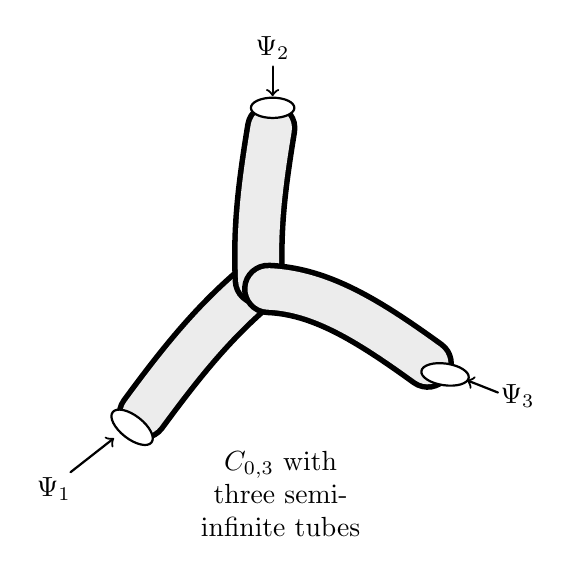
\begin{tikzpicture}[scale=0.92, line cap=round, line join=round]
\draw[line width=19pt, black]
  (0.05,0.05) .. controls (-0.55,-0.45) and (-1.00,-1.00) .. (-1.55,-1.75);
\draw[line width=15pt, gray!15]
  (0.05,0.05) .. controls (-0.55,-0.45) and (-1.00,-1.00) .. (-1.55,-1.75);

\draw[line width=19pt, black]
  (0.05,0.10) .. controls (0.02,0.80) and (0.08,1.35) .. (0.22,2.20);
\draw[line width=15pt, gray!15]
  (0.05,0.10) .. controls (0.02,0.80) and (0.08,1.35) .. (0.22,2.20);

\draw[line width=19pt, black]
  (0.18,-0.02) .. controls (0.90,-0.05) and (1.55,-0.45) .. (2.38,-1.05);
\draw[line width=15pt, gray!15]
  (0.18,-0.02) .. controls (0.90,-0.05) and (1.55,-0.45) .. (2.38,-1.05);

\fill[white] (-1.70,-1.93) ellipse [x radius=0.34, y radius=0.16, rotate=-38];
\draw[thick] (-1.70,-1.93) ellipse [x radius=0.34, y radius=0.16, rotate=-38];
\fill[white] (0.24,2.48) ellipse [x radius=0.30, y radius=0.14];
\draw[thick] (0.24,2.48) ellipse [x radius=0.30, y radius=0.14];
\fill[white] (2.62,-1.20) ellipse [x radius=0.33, y radius=0.15, rotate=-8];
\draw[thick] (2.62,-1.20) ellipse [x radius=0.33, y radius=0.15, rotate=-8];

\draw[->, thick] (-2.55,-2.55) -- (-1.95,-2.08);
\draw[->, thick] (0.24,3.05) -- (0.24,2.64);
\draw[->, thick] (3.35,-1.45) -- (2.92,-1.28);
\node at (-2.78,-2.78) {$\Psi_1$};
\node at (0.24,3.30) {$\Psi_2$};
\node at (3.62,-1.50) {$\Psi_3$};
\node[align=center, text width=2.6cm] at (0.35,-2.85) {$C_{0,3}$ with three semi-infinite tubes};
\end{tikzpicture}
\end{minipage}
\hfill
\begin{minipage}{0.46\textwidth}
\centering
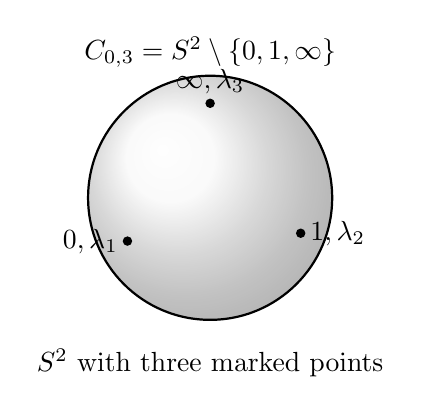
\begin{tikzpicture}[scale=1.0, line cap=round, line join=round]
\shade[ball color=gray!12, opacity=0.45] (0,0) circle (1.55);
\draw[thick] (0,0) circle (1.55);
\fill (0,1.2) circle (0.06);
\fill (-1.05,-0.55) circle (0.06);
\fill (1.15,-0.45) circle (0.06);
\node[above] at (0,1.2) {$\infty,\lambda_3$};
\node[left] at (-1.05,-0.55) {$0,\lambda_1$};
\node[right] at (1.15,-0.45) {$1,\lambda_2$};
\node at (0,-2.1) {$S^2$ with three marked points};
\node at (0,1.85) {$C_{0,3}=S^2\setminus\{0,1,\infty\}$};
\end{tikzpicture}
\end{minipage}
\caption{Two equivalent target-space pictures for the next exact-orbifold observable. Because the Poisson/BF core forgets the target Weyl representative, the three-punctured sphere $C_{0,3}$ may be viewed either as a pair of pants with three semi-infinite cylinders carrying general asymptotic states $\Psi_i$, or as the compact sphere with three marked points labeled by ramification profiles $\lambda_i$. Each $\Psi_i$ may represent a multi-string state with profile $\lambda_i$; the single-cycle case is the special choice $\lambda_i=(w_i)$.}
\label{fig:pair-of-pants-target}
\end{figure}

A general exact-orbifold state on one tube need not be a single long string; it can carry an arbitrary cycle decomposition
\begin{equation}\label{eq:ramification-profile}
\lambda_i=(w_{i,1},\dots,w_{i,\ell_i}),
\qquad
\sum_{a=1}^{\ell_i} w_{i,a}\le N,
\end{equation}
so the most general tree-level observable is a three-point amplitude between states of prescribed ramification profile on the three tubes. In the present note I restrict attention to the simplest nontrivial case in which each external state is a single-cycle twisted-sector state, so each profile is a one-part partition $\lambda_i=(w_i)$. After compactifying the cylindrical ends back to the marked points $(0,1,\infty)$ on $S^2$, this is equivalently the canonical three-point function of single-cycle twist operators.

\subsection{Exact Orbifold Three-Point Input}

At the orbifold point, define the normalized single-cycle class operator by
\begin{equation}\label{eq:class-operator}
\widehat{\sigma}_{[w]}
:=
\frac{1}{\sqrt{|[w]|_N}}
\sum_{g\in [w]}\sigma_g,
\qquad
|[w]|_N=\frac{N!}{w(N-w)!},
\end{equation}
where $[w]\subset S_N$ is the conjugacy class of $w$-cycles. For the connected three-point function associated with degree-$d$ covers of genus $g$, the standard covering-space description of symmetric-product orbifolds takes the form \cite{arutyunov1998orbifoldscattering,lunin2001correlationorbifolds,lunin2002threepointorbifolds,pakman2009diagramssymmetricorbifold,pakman2009extremalhurwitz}
\begin{equation}\label{eq:orbifold-three-point}
\mc C_{123}^{(g)}(N)
:=
\left\langle
\widehat{\sigma}_{[w_1]}(0)\,
\widehat{\sigma}_{[w_2]}(1)\,
\widehat{\sigma}_{[w_3]}(\infty)
\right\rangle_{g}^{\mathrm{conn}}
=
\frac{N!}{(N-d)!}\,
\frac{
H_d^{(g)}(w_1,w_2,w_3)\,
\mc C_{\mathrm{seed}}^{(g)}(w_1,w_2,w_3)
}{
\sqrt{|[w_1]|_N\,|[w_2]|_N\,|[w_3]|_N}
}.
\end{equation}
Here $d$ is the number of active copies. In the present note I will simply \emph{quote} the exact orbifold formula \eqref{eq:orbifold-three-point} rather than rederive it. The underlying covering-space derivation, including the Liouville/conformal-anomaly contribution and the normalization of bosonic twist operators, is carried out explicitly in \cite[Secs.~5--6]{lunin2001correlationorbifolds}. For the supersymmetric single-cycle chiral operators relevant here, \cite[Sec.~4]{lunin2002threepointorbifolds} writes the normalized three-point function as a ratio of current/spin-field correlators on the cover multiplied by the exponential of a difference of Liouville actions, with the Liouville part identified with the bosonic twist contribution from \cite{lunin2001correlationorbifolds}. The later diagrammatic/Hurwitz reorganization is reviewed in \cite{pakman2009diagramssymmetricorbifold}. In this quoted orbifold formula, $H_d^{(g)}$ should be understood as the weighted Hurwitz count
\begin{equation}\label{eq:weighted-hurwitz-count}
H_d^{(g)}(w_1,w_2,w_3)
:=
\sum_{[f]}
\frac{1}{|\mathrm{Aut}(f)|},
\end{equation}
while $\mc C_{\mathrm{seed}}^{(g)}$ denotes the reduced seed-theory factor appearing in that quoted orbifold result. The important point for the present note is that \eqref{eq:orbifold-three-point} is an orbifold-side input imported from the literature; its string-side analogue is part of what must be checked rather than assumed. For three branch points, the degree is constrained by Riemann--Hurwitz:
\begin{equation}\label{eq:riemann-hurwitz-three-point}
2-2g
=
2d-\sum_{i=1}^3 (w_i-1),
\qquad
d=\frac{w_1+w_2+w_3-1}{2}-g.
\end{equation}
In particular, for fixed cycle lengths $(w_1,w_2,w_3)$ and large $N$, the leading contribution comes from $g=0$. Writing
\begin{equation}\label{eq:tree-level-degree}
d_0:=\frac{w_1+w_2+w_3-1}{2},
\end{equation}
one finds directly from \eqref{eq:orbifold-three-point} that
\begin{equation}\label{eq:orbifold-three-point-leading}
\mc C_{123}^{(0)}(N)
=
N^{-1/2}
\Big[
\sqrt{w_1w_2w_3}\,
H_{d_0}^{(0)}(w_1,w_2,w_3)\,
\mc C_{\mathrm{seed}}^{(0)}(w_1,w_2,w_3)
+O(N^{-1})
\Big].
\end{equation}
\bluecomment{Equation \eqref{eq:orbifold-three-point-leading} is the dilute large-$N$ regime with fixed cycle lengths $(w_1,w_2,w_3)$ as $N\to\infty$. A macroscopic-winding regime would require a separate asymptotic analysis and is not covered by the present tree-level comparison.}
Thus the first nontrivial large-$N$ comparison is indeed a genuine tree-level worldsheet problem: the leading orbifold coefficient comes from genus-zero covers and scales as $N^{-1/2}$.

It is worth emphasizing that the factor $\sqrt{w_1w_2w_3}$ in \eqref{eq:orbifold-three-point-leading} is already a nontrivial structural fact. A priori the leading normalization of the orbifold three-point function could have been an arbitrary joint function of $(w_1,w_2,w_3)$. Instead, the exact orbifold answer organizes itself so that the leading local normalization factorizes puncture-by-puncture,
\[
\sqrt{w_1w_2w_3}=\prod_{i=1}^3 \sqrt{w_i}.
\]
This is precisely the pattern suggested by the rigid pair-of-pants worldsheet picture, where one would expect the leading local normalization to be attached independently to the three asymptotic tubes. Of course this factorization does \emph{not} trivialize the full correlator: the Hurwitz multiplicity $H_{d_0}^{(0)}(w_1,w_2,w_3)$ and the reduced seed-theory factor $\mc C_{\mathrm{seed}}^{(0)}(w_1,w_2,w_3)$ remain genuinely collective data of the whole three-point function. The point is only that the exact orbifold result already exhibits the puncture-local factorization pattern that the worldsheet construction would naturally predict for the leading normalization sector.

This is the right exact-orbifold observable to compare to the first-order string beyond genus one. It is already a canonical fixed-$N$ quantity, so unlike the torus free energy it does not structurally require a grand-canonical fugacity. One may still study its large-$N$ asymptotic expansion, but that expansion is part of the exact $\Sym^N(\bR^8)$ CFT itself. Grand-canonical generating functions may be useful for organizing an infinite family of such correlators, but they are optional bookkeeping rather than part of the definition of one fixed three-point function.

\subsection{Worldsheet-CFT Setup on \texorpdfstring{$C_{0,3}$}{C0,3}}

On the worldsheet side, the tree-level problem should likewise be formulated on the punctured target $C_{0,3}$ with specified asymptotic states on its three cylindrical ends. On the orbifold side, compactifying the $i$-th tube back to a marked point produces the exact-orbifold state space $\mc H^{\rm orb}_{\lambda_i}$ with ramification profile $\lambda_i$. On the string side, the corresponding object should be an asymptotic state space $\mc H^{\rm str}_{z_i}$ attached to the $i$-th cylindrical end of $C_{0,3}$. A precise duality statement at this level would therefore require maps
\begin{equation}\label{eq:tube-state-dictionary}
\iota_i:\mc H^{\rm orb}_{\lambda_i}\to \mc H^{\rm str}_{z_i},
\end{equation}
so that an orbifold state $\Psi_i^{\rm orb}\in \mc H^{\rm orb}_{\lambda_i}$ is compared to the corresponding asymptotic string state $\Psi_i:=\iota_i(\Psi_i^{\rm orb})\in \mc H^{\rm str}_{z_i}$. In the present note I keep this dictionary formal and use $\Psi_i$ for the string-side asymptotic state. The corresponding string observable should be a trilinear pairing
\begin{equation}\label{eq:pair-of-pants-amplitude}
\mc A^{\rm str}_{C_{0,3}}(\Psi_1,\Psi_2,\Psi_3),
\end{equation}
defined by the first-order worldsheet path integral over maps to $C_{0,3}$ whose asymptotics on the preimages of the three target tubes encode the states $\Psi_i$.
Expressed in the language of the worldsheet CFT, the tree-level object one wants is a sphere correlator of three BRST vertex operators in the fixed target background $C_{0,3}$. Formally, after choosing superghost pictures $(q_i,\bar q_i)$ with
\begin{equation}\label{eq:picture-balance}
q_1+q_2+q_3=-2,
\qquad
\bar q_1+\bar q_2+\bar q_3=-2,
\end{equation}
and fixing the worldsheet punctures $\zeta_i$ by the $\mathrm{PSL}(2,\bC)$ automorphism of $\Sigma\simeq S^2$, one would write
\begin{equation}\label{eq:pair-of-pants-cft-correlator}
\mc A^{\rm str}_{C_{0,3}}(\Psi_1,\Psi_2,\Psi_3)
=
\sum_{\mathfrak s}
\left\langle
c_{\rm gh}\tilde c_{\rm gh}\,\mc V_{\Psi_1,\mathfrak s}^{(q_1,\bar q_1)}(\zeta_1,\bar\zeta_1)\,
c_{\rm gh}\tilde c_{\rm gh}\,\mc V_{\Psi_2,\mathfrak s}^{(q_2,\bar q_2)}(\zeta_2,\bar\zeta_2)\,
c_{\rm gh}\tilde c_{\rm gh}\,\mc V_{\Psi_3,\mathfrak s}^{(q_3,\bar q_3)}(\zeta_3,\bar\zeta_3)
\right\rangle_{\Sigma=S^2,\mathfrak s}.
\end{equation}
Here $\mathfrak s$ labels the map sector of the worldsheet CFT in the fixed target background $C_{0,3}$, $c_{\rm gh},\tilde c_{\rm gh}$ are the usual reparametrization ghosts, and $\mc V_{\Psi_i,\mathfrak s}^{(q_i,\bar q_i)}$ denotes the BRST vertex operator corresponding to the asymptotic target-tube state $\Psi_i$. For the three-point sphere amplitude there is no residual worldsheet moduli integral after fixing $(\zeta_1,\zeta_2,\zeta_3)$, so the only remaining sum is over the allowed map sectors $\mathfrak s$. What is not yet known in the present note is the explicit construction of these longitudinal vertex operators in the curved first-order system and the proof that the relevant sectors $\mathfrak s$ are precisely the branched-cover sectors described below.

For the lowest supersymmetric single-cycle states, a natural standard choice is the NS--NS sphere picture assignment
\begin{equation}\label{eq:sphere-picture-choice}
(q_1,\bar q_1)=(q_2,\bar q_2)=(-1,-1),
\qquad
(q_3,\bar q_3)=(0,0),
\end{equation}
which obeys \eqref{eq:picture-balance}. I will use this choice below whenever I discuss candidate explicit sphere vertices.

For the standard punctures $(z_1,z_2,z_3)=(0,1,\infty)$, the GitHub draft also makes the concrete tube-coordinate choice
\begin{equation}\label{eq:explicit-three-tube-coordinates}
\xi_1=-\log z,
\qquad
\xi_2=-\log(z-1),
\qquad
\xi_3=\log z=-\log(1/z),
\end{equation}
and likewise antiholomorphically. This is just a concrete specialization of \eqref{eq:target-tube-coordinate}, but it is helpful when writing explicit puncture operators.

To make the asymptotic state more concrete, choose near the $i$-th target puncture the standard cylindrical coordinate
\begin{equation}\label{eq:target-tube-coordinate}
\xi_i=s_i+i\phi_i:=-\log(z-z_i),
\qquad
\phi_i\sim \phi_i+2\pi.
\end{equation}
The angular variable $\phi_i$ is the circle coordinate of the semi-infinite target tube. The simplest nontrivial asymptotic state on that tube is then a \emph{single-string winding state} $\Psi_{w_i}$ with profile $\lambda_i=(w_i)$: in the corresponding classical sector, one local worldsheet coordinate $t_i$ obeys
\begin{equation}\label{eq:single-string-tube-winding}
z-z_i=t_i^{\,w_i}
\qquad\Longleftrightarrow\qquad
\xi_i=-\,w_i\log t_i.
\end{equation}
Thus going once around the worldsheet preimage $t_i\mapsto e^{2\pi i}t_i$ shifts the target-tube angle by $\phi_i\mapsto \phi_i+2\pi w_i$. In this precise sense the state $\Psi_{w_i}$ is a winding-$w_i$ string state with respect to the circle of the $i$-th target tube. This should not be confused with the flat-torus benchmark of Section~6, where the relevant circle is an actual global target-space circle of $C=T^2$; here the tube circle is only a local representative of the puncture on $C_{0,3}$. The canonical three-point coefficient \eqref{eq:orbifold-three-point} corresponds to choosing the lowest such single-string states, which compactify to the class-normalized single-cycle twist operators $\widehat{\sigma}_{[w_i]}$.

At the level of asymptotic Hilbert spaces, the simplest candidate single-string state should therefore take the tensor-product form
\begin{equation}\label{eq:single-string-state-factorization}
\left|\Psi_{w_i,\chi_i}\right\rangle_i
=
\left|w_i\right\rangle_i^{\rm long}\otimes \left|\chi_i\right\rangle_i^\perp
\in
\mc H^{\rm str}_{z_i},
\end{equation}
where $\left|w_i\right\rangle_i^{\rm long}$ is the lowest longitudinal state in the winding-$w_i$ sector of the $i$-th target tube and $\left|\chi_i\right\rangle_i^\perp$ is a state of the transverse $\bR^8$ SCFT. When the transverse seed state is fixed once and for all, I abbreviate $\Psi_{w_i,\chi_i}$ to $\Psi_{w_i}$. Equation \eqref{eq:single-string-state-factorization} should be understood as the asymptotic-state ansatz suggested by the target-tube geometry; the explicit curved-background construction of $\left|w_i\right\rangle_i^{\rm long}$ remains open.

If a BRST-complete worldsheet construction exists, the corresponding unintegrated closed-string state should be represented by a BRST class
\begin{equation}\label{eq:single-string-brst-class}
\big[c_{\rm gh}\tilde c_{\rm gh}\,\mc V^{(q_i,\bar q_i)}_{w_i,\chi_i}\big]
\in
H^2_{\rm BRST}(C_{0,3}),
\end{equation}
where $\chi_i$ denotes the chosen transverse seed state and $(q_i,\bar q_i)$ obey the picture constraint \eqref{eq:picture-balance}. The longitudinal content of $\mc V^{(q_i,\bar q_i)}_{w_i,\chi_i}$ should then be characterized locally by the tube-winding OPE
\begin{equation}\label{eq:tube-winding-ope}
\partial \xi_i\!\big(X^+(t)\big)\,
\mc V^{(q_i,\bar q_i)}_{w_i,\chi_i}(0)
\sim
-\,\frac{w_i}{t}\,
\mc V^{(q_i,\bar q_i)}_{w_i,\chi_i}(0)
\qquad
\text{and}
\qquad
\bar\partial \bar\xi_i\!\big(X^-(\bar t)\big)\,
\mc V^{(q_i,\bar q_i)}_{w_i,\chi_i}(0)
\sim
-\,\frac{w_i}{\bar t}\,
\mc V^{(q_i,\bar q_i)}_{w_i,\chi_i}(0),
\end{equation}
equivalently by the contour-charge condition
\begin{equation}\label{eq:tube-winding-charge}
W_i\,\mc V^{(q_i,\bar q_i)}_{w_i,\chi_i}
:=
-\,\frac{1}{2\pi i}\oint \partial \xi_i\!\big(X^+\big)\,
\mc V^{(q_i,\bar q_i)}_{w_i,\chi_i}
=
w_i\,\mc V^{(q_i,\bar q_i)}_{w_i,\chi_i},
\end{equation}
and likewise antiholomorphically. Equation \eqref{eq:tube-winding-ope} is simply the operator-language version of \eqref{eq:single-string-tube-winding}. What remains open is the explicit realization of such operators in the curved first-order CFT and their normalization.

\subsection{Candidate Explicit Longitudinal Operators}

The new GitHub draft suggests a concrete candidate for the previously abstract longitudinal ramification operator. To avoid confusion with the reparametrization ghosts, in this subsection I temporarily rename the longitudinal matter fermions by
\begin{equation}\label{eq:longitudinal-fermion-rename}
\psi^+:=c,
\qquad
\rho:=b,
\qquad
\bar\psi^-:=\bar c,
\qquad
\bar\rho:=\bar b.
\end{equation}
Thus $(\gamma,\beta)$ and $(\psi^+,\rho)$ are the longitudinal matter fields, while $(c_{\rm gh},b_{\rm gh})$ and the bosonized superghosts belong to the usual RNS ghost sector.

It is worth making the logic of the GitHub construction explicit, because the operator below was found by a constrained covariantization rather than by an independent derivation of the curved BRST cohomology. In flat space, Gomis and Ooguri use a winding insertion built from $\gamma$, $\bar\gamma$, and line integrals of $\beta$, $\bar\beta$ whose formal OPEs reproduce the desired logarithmic monodromy \cite[Sec.~5]{gomis2000nonrelativisticclosedstringtheory}. The curved-target problem is then: replace the bare first-order fields by objects that patch tensorially on $C$, while still producing the local tube-winding behavior \eqref{eq:tube-winding-ope}--\eqref{eq:tube-winding-charge}. The candidate below is the simplest operator that simultaneously tries to satisfy those two requirements.
\bluecomment{The logical gap is therefore precise. Matching the flat Gomis--Ooguri template, target-space covariance, and the desired \emph{formal local} OPEs does not yet prove that one has constructed the correct globally defined quantum BRST vertex in the curved theory. What is still missing is the passage from this reverse-engineered ansatz to a theorem-level operator statement: path independence, locality, conformal weight, BRST closure, and harmless picture changing.}

Guided by the curved patching formulas and by the flat Gomis--Ooguri winding operator, a natural tensorial building block is the covariant momentum
\begin{equation}\label{eq:candidate-covariant-momentum}
\Pi_u:=\beta_u-\Gamma_u\,\rho_u\psi_u^+,
\qquad
\bar\Pi_{\bar u}:=\bar\beta_{\bar u}-\bar\Gamma_{\bar u}\,\bar\rho_{\bar u}\bar\psi_{\bar u}^-,
\qquad
\Gamma_u:=2\partial_u\omega,
\end{equation}
\bluecomment{Equation \eqref{eq:candidate-covariant-momentum} itself is just a proposed definition of a covariant composite operator. What is not yet proved is that this is the correct globally defined quantum operator with the required tensorial patching and overlap properties in the curved first-order CFT.}
for a local target metric representative $ds_C^2=e^{2\omega}du\,d\bar u$. In a tube chart one may then define the corresponding tube components
\begin{equation}\label{eq:candidate-covariant-components}
\Pi_{\xi_i}:=\frac{\partial u}{\partial \xi_i}\,\Pi_u,
\qquad
\bar\Pi_{\bar\xi_i}:=\frac{\partial \bar u}{\partial \bar\xi_i}\,\bar\Pi_{\bar u}.
\end{equation}
The GitHub draft further emphasizes that if one chooses the auxiliary Hermitian representative $ds_C^2=d\xi_i\,d\bar\xi_i$ in a tube chart, then $\Gamma_{\xi_i}=0$ and $\Pi_{\xi_i}$ reduces locally to the bare first-order field $\beta_{\xi_i}$. This is the precise local sense in which the proposed curved operator is meant to reduce to the flat Gomis--Ooguri winding insertion.
\bluecomment{This local reduction is very plausible and is useful intuition, but in the present note it still depends on the unproved tensorial/operator-level status of \eqref{eq:candidate-covariant-momentum}.}

Using these covariant components, a natural candidate ramification insertion at the worldsheet point $x_i$ is
\begin{equation}\label{eq:candidate-ramification-operator}
\Sigma^{\rm long,cand}_{w_i,\nu_i,\bar\nu_i}(x_i,\bar x_i)
:=
\mc N_{w_i}
:\exp\!\Big[
i\bar\nu_i\,\xi_i\!\big(X^+(x_i,\bar x_i)\big)
-w_i\!\int^{x_i}\!\Pi_{\xi_i}
+i\nu_i\,\bar\xi_i\!\big(X^-(x_i,\bar x_i)\big)
-w_i\!\int^{\bar x_i}\!\bar\Pi_{\bar\xi_i}
\Big]:,
\end{equation}
\bluecomment{This line-integral operator is only a candidate. Path independence, branch-cut independence, locality, mutual monodromy with other insertions, and BRST closure are all still unproved.}
with lowest candidate state
\begin{equation}\label{eq:candidate-lowest-longitudinal-state}
\Sigma^{\rm long,cand}_{w_i}:=
\Sigma^{\rm long,cand}_{w_i,0,0}.
\end{equation}
The GitHub draft further spells out the formal local OPE package of this operator as
\begin{equation}\label{eq:candidate-longitudinal-local-opes}
\begin{aligned}
\xi_i\!\big(X^+(t,\bar t)\big)\,\Sigma^{\rm long,cand}_{w_i,\nu_i,\bar\nu_i}(x_i,\bar x_i)
&\sim
-\,w_i\log(t-x_i)\,\Sigma^{\rm long,cand}_{w_i,\nu_i,\bar\nu_i}(x_i,\bar x_i),
\\
\Pi_{\xi_i}(t)\,\Sigma^{\rm long,cand}_{w_i,\nu_i,\bar\nu_i}(x_i,\bar x_i)
&\sim
\frac{i\bar\nu_i}{t-x_i}\,
\Sigma^{\rm long,cand}_{w_i,\nu_i,\bar\nu_i}(x_i,\bar x_i),
\end{aligned}
\end{equation}
with the analogous antiholomorphic formulas for $\bar\xi_i(X^-)$ and $\bar\Pi_{\bar\xi_i}$. For $\nu_i=\bar\nu_i=0$, differentiating the first line reproduces \eqref{eq:tube-winding-ope}.
\bluecomment{Equation \eqref{eq:candidate-longitudinal-local-opes} is part of the stronger GitHub-draft package. In the present note it is still only a formal free-field consequence of the candidate operator, not a theorem-level OPE computation in the curved BRST theory.}
Formally, treating \eqref{eq:candidate-ramification-operator} by the same free-field manipulations as in the flat first-order system, one indeed reproduces the desired local monodromy conditions \eqref{eq:tube-winding-ope}--\eqref{eq:tube-winding-charge}. This is the main reason the candidate is attractive: it is the curved analogue of the flat winding insertion and it already has the puncture-local structure suggested by the factorized $\prod_i\sqrt{w_i}$ in \eqref{eq:orbifold-three-point-leading}.

Under the same formal assumptions, the natural lowest NS--NS candidate vertex would be
\begin{equation}\label{eq:candidate-ns-vertex}
\mc V^{(-1,-1),{\rm cand}}_{w_i,\chi_i}
:=
\Sigma^{\rm long,cand}_{w_i}\,
e^{-\varphi-\bar\varphi}\,
\mc O_{\chi_i}^\perp,
\end{equation}
\bluecomment{Before this can be accepted as a genuine sphere vertex operator, one still needs an explicit conformal-weight check, a BRST-closure check, and a proof that picture changing does not generate extra longitudinal contributions.}
where $\mc O_{\chi_i}^\perp$ is the chosen one-copy transverse seed operator of weights $(\tfrac12,\tfrac12)$. With the sphere picture choice \eqref{eq:sphere-picture-choice}, one would then use two insertions of \eqref{eq:candidate-ns-vertex} and one standard picture-changed representative.
The corresponding stronger $(0,0)$-picture candidate used in the GitHub draft is
\begin{equation}\label{eq:candidate-zero-picture}
\mc V^{(0,0),{\rm cand}}_{w_i,\chi_i}
:=
\mc X_{\rm PCO}\,\bar{\mc X}_{\rm PCO}\cdot
\mc V^{(-1,-1),{\rm cand}}_{w_i,\chi_i},
\qquad
\mc X_{\rm PCO}:=\{Q,\xi_{\gh}\},
\qquad
\bar{\mc X}_{\rm PCO}:=\{\bar Q,\bar\xi_{\gh}\}.
\end{equation}
\bluecomment{The PCO in \eqref{eq:candidate-zero-picture} is the standard NSR picture-changing operator, and \eqref{eq:candidate-zero-picture} is therefore just an abstract definition of a candidate $(0,0)$ representative. What is still open is the extraction of a more explicit local operator formula for that representative in the curved longitudinal theory, which would require the relevant OPE with the curved longitudinal supercurrent.}

At present, however, \eqref{eq:candidate-ramification-operator} should be regarded only as a candidate, not as an established BRST vertex. To upgrade it to a theorem-level construction, one would still need to show at least:
\begin{equation}\label{eq:candidate-vertex-checklist}
\begin{aligned}
&\text{(i) independence of the chosen branch-cut network and integration paths,}\\
&\text{(ii) correct conformal weights and BRST closure,}\\
&\text{(iii) locality and mutual monodromy with other insertions,}\\
&\text{(iv) that picture changing introduces no extra longitudinal terms.}
\end{aligned}
\end{equation}
For that reason I will use $\Sigma^{\rm long,cand}$ only as concrete guidance, while keeping the main localization formulas below in the theorem-neutral notation $\mc V^{\rm PSM}_{w_i;f}$.

\subsection{Branched-Cover Localization}

After compactifying the target tubes back to the marked points $(0,1,\infty)$, the asymptotic data become ramification data. For a general multi-string state, the puncture at $z_i$ carries the profile $\lambda_i=(w_{i,1},\dots,w_{i,\ell_i})$, so the compactified map has local behavior
\begin{equation}\label{eq:local-branching-profile}
z-z_i=t_{i,a}^{\,w_{i,a}},
\qquad
a=1,\dots,\ell_i.
\end{equation}
Thus there are $\ell_i$ preimages above the $i$-th puncture, one for each constituent long string in the target-tube state. In the single-cycle case $\lambda_i=(w_i)$ studied here, there is only one preimage above each puncture and \eqref{eq:local-branching-profile} reduces to
\begin{equation}\label{eq:local-branching}
z-z_i=t_i^{\,w_i}.
\end{equation}
The lifted longitudinal field is then single-valued in $t_i$. The classical saddles are therefore naturally organized by holomorphic branched covers
\begin{equation}\label{eq:branched-cover-worldsheet}
f:\Sigma\to S^2
\end{equation}
with ramification data fixed by the three profiles $\lambda_i$. In the single-cycle case this specializes to $(w_1,w_2,w_3)$ with degree constrained by \eqref{eq:riemann-hurwitz-three-point}. For three marked points on $\Sigma=S^2$, there is no continuous modulus after fixing the insertion points to $(0,1,\infty)$, so the classical localization problem is a discrete sum over Hurwitz classes rather than a higher-dimensional moduli integral. Thus the branched-cover language should be understood as the compactified version of a pair-of-pants amplitude with asymptotic string states on the three target tubes.
Figure~\ref{fig:branched-cover-data} illustrates the passage from target ramification profiles to preimages on the covering worldsheet.

\begin{figure}[t]
\centering
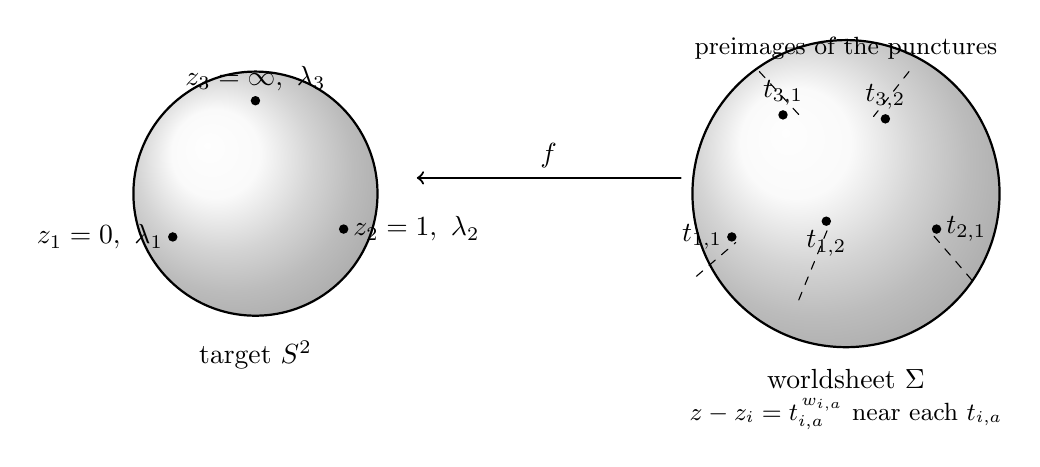
\begin{tikzpicture}[scale=1.0, line cap=round, line join=round]
\shade[ball color=gray!10, opacity=0.5] (-4.3,0) circle (1.55);
\draw[thick] (-4.3,0) circle (1.55);
\fill (-4.3,1.18) circle (0.06);
\fill (-5.35,-0.55) circle (0.06);
\fill (-3.18,-0.45) circle (0.06);
\node[above] at (-4.3,1.18) {$z_3=\infty,\ \lambda_3$};
\node[left] at (-5.35,-0.55) {$z_1=0,\ \lambda_1$};
\node[right] at (-3.18,-0.45) {$z_2=1,\ \lambda_2$};
\node at (-4.3,-2.05) {target $S^2$};

\shade[ball color=gray!10, opacity=0.5] (3.2,0) circle (1.95);
\draw[thick] (3.2,0) circle (1.95);
\fill (2.4,1.0) circle (0.06);
\fill (3.7,0.95) circle (0.06);
\fill (1.75,-0.55) circle (0.06);
\fill (2.95,-0.35) circle (0.06);
\fill (4.35,-0.45) circle (0.06);
\node[above] at (2.4,1.0) {$t_{3,1}$};
\node[above] at (3.7,0.95) {$t_{3,2}$};
\node[left] at (1.75,-0.55) {$t_{1,1}$};
\node[below] at (2.95,-0.35) {$t_{1,2}$};
\node[right] at (4.35,-0.45) {$t_{2,1}$};
\node at (3.2,-2.35) {worldsheet $\Sigma$};
\draw[->, thick] (1.1,0.2) -- (-2.25,0.2) node[midway, above] {$f$};

\draw[dashed] (2.1,1.55) -- (2.65,0.95);
\draw[dashed] (4.0,1.55) -- (3.55,0.98);
\draw[dashed] (1.3,-1.05) -- (1.8,-0.62);
\draw[dashed] (2.6,-1.35) -- (2.98,-0.42);
\draw[dashed] (4.8,-1.1) -- (4.3,-0.52);
\node at (3.2,1.85) {\small preimages of the punctures};
\node at (3.2,-2.8) {\small $z-z_i=t_{i,a}^{\,w_{i,a}}$ near each $t_{i,a}$};
\end{tikzpicture}
\caption{Compactified branched-cover picture for the pair-of-pants amplitude. A target puncture with profile $\lambda_i=(w_{i,1},\dots,w_{i,\ell_i})$ has $\ell_i$ preimages on the worldsheet, one for each constituent long string in the asymptotic state on the $i$-th tube. In the single-cycle case used for \eqref{eq:orbifold-three-point} and \eqref{eq:orbifold-three-point-leading}, each $\lambda_i=(w_i)$ and there is only one preimage above each puncture.}
\label{fig:branched-cover-data}
\end{figure}

Schematically, the desired string calculation should take the form
\begin{equation}\label{eq:pair-of-pants-localized}
\mc A^{\rm str}_{C_{0,3}}(\Psi_1,\Psi_2,\Psi_3)
=
\sum_{[f]\in \mathrm{Hurwitz}(\lambda_1,\lambda_2,\lambda_3)}
\mc W_f(\Psi_1,\Psi_2,\Psi_3),
\end{equation}
\bluecomment{The branched-cover sum is the expected localized form, but the exact identification of worldsheet sectors with Hurwitz classes and the precise BRST-complete cover weight are not yet derived.}
where the sum runs over compactified branched-cover classes compatible with the three asymptotic tube states and $\mc W_f$ is the full BRST-complete weight of the cover, including vertex-operator normalization, ghost insertions, nonzero-mode determinants, and the transverse seed correlator on the covering surface. In the single-cycle case, after choosing the external states corresponding to the class-normalized twist operators of \eqref{eq:class-operator}, the target quantity to reproduce is precisely \eqref{eq:orbifold-three-point}.
The GitHub draft makes the stronger claim that once the explicit ramification operator is accepted, the sector sum in \eqref{eq:pair-of-pants-cft-correlator} is \emph{precisely} the Hurwitz sum \eqref{eq:pair-of-pants-localized}.
\bluecomment{That stronger identification is not yet established in the present note. It depends on the unresolved locality/BRST issues of the candidate operator and on the exact localization measure.}

For the leading single-cycle genus-zero comparison, one can write the same prescription more explicitly. A cover $[f]\in \mathrm{Hurwitz}_0(d_0;w_1,w_2,w_3)$ has a unique ramification point $x_i\in \Sigma\simeq S^2$ above each puncture $z_i$, and the fixed-cover contribution should be the sphere correlator
\begin{equation}\label{eq:fixed-cover-correlator}
\mc A^{\rm str,(0)}_{123}[f]
:=
\left\langle
c_{\rm gh}\tilde c_{\rm gh}\,\mc V^{(q_1,\bar q_1)}_{w_1,\chi_1;f}(x_1,\bar x_1)\,
c_{\rm gh}\tilde c_{\rm gh}\,\mc V^{(q_2,\bar q_2)}_{w_2,\chi_2;f}(x_2,\bar x_2)\,
c_{\rm gh}\tilde c_{\rm gh}\,\mc V^{(q_3,\bar q_3)}_{w_3,\chi_3;f}(x_3,\bar x_3)
\right\rangle_{\Sigma=S^2,f},
\end{equation}
with no additional worldsheet moduli integral after the three insertions are fixed. Formally one expects the fixed-cover vertex operator to factor as
\begin{equation}\label{eq:fixed-cover-vertex-factorization}
\mc V^{(q_i,\bar q_i)}_{w_i,\chi_i;f}
=
\mc V^{\rm long}_{w_i;f}\,
\mc U^\perp_{\chi_i}\,
e^{q_i\varphi+\bar q_i\bar\varphi},
\end{equation}
where $\mc U^\perp_{\chi_i}$ is the transverse seed-state operator on the covering sphere, $e^{q_i\varphi+\bar q_i\bar\varphi}$ is the usual superghost factor, and the unresolved ingredient is the longitudinal ramification operator $\mc V^{\rm long}_{w_i;f}$ together with its normalization in the curved first-order background. In this notation, the weight appearing in \eqref{eq:pair-of-pants-localized} is simply
\begin{equation}\label{eq:fixed-cover-weight}
\mc W_f(\Psi_{w_1,\chi_1},\Psi_{w_2,\chi_2},\Psi_{w_3,\chi_3})
=
\frac{1}{|\mathrm{Aut}(f)|}\,
\mc A^{\rm str,(0)}_{123}[f].
\end{equation}
For the sphere three-point function the standard tree-level prescription is already maximally simple: there are no integrated vertices because
\begin{equation}\label{eq:sphere-three-point-no-moduli}
\dim_{\bC}\mc M_{0,3}=0,
\qquad
n_{\mathrm{int}}=3-3=0.
\end{equation}
Thus \eqref{eq:fixed-cover-correlator} already is the complete fixed-cover worldsheet prescription once the three local BRST operators are known. Equivalently, by radial quantization around a small circle on $\Sigma_f$ centered at the ramification point $x_i$, the local insertion defines a BRST state
\begin{equation}\label{eq:fixed-cover-local-state}
\left|\Psi_{w_i,\chi_i};f,x_i\right\rangle
:=
\lim_{\zeta\to x_i}
c_{\rm gh}\tilde c_{\rm gh}\,
\mc V^{(q_i,\bar q_i)}_{w_i,\chi_i;f}(\zeta,\bar\zeta)
\left|0\right\rangle_{\Sigma_f}
\in
\mc H_{\rm BRST}^{\rm ws}(x_i;f),
\end{equation}
and the fixed-cover amplitude is the induced trilinear pairing of these three local BRST states. In this form the only missing data are no longer kinematic or measure-theoretic on the sphere; they are entirely concentrated in the explicit construction and normalization of the longitudinal ramification operators.

With the specific picture choice \eqref{eq:sphere-picture-choice}, the GitHub draft specializes \eqref{eq:fixed-cover-correlator} to
\begin{equation}\label{eq:fixed-cover-correlator-sphere-choice}
\begin{aligned}
\mc A^{\rm str,(0)}_{123}[f]
&=
\Big\langle
c_{\rm gh}\tilde c_{\rm gh}\,\mc V^{(-1,-1)}_{w_1,\chi_1;f}(x_1,\bar x_1)\,
c_{\rm gh}\tilde c_{\rm gh}\,\mc V^{(-1,-1)}_{w_2,\chi_2;f}(x_2,\bar x_2)\,
\\
&\hspace{2cm}
c_{\rm gh}\tilde c_{\rm gh}\,\mc V^{(0,0)}_{w_3,\chi_3;f}(x_3,\bar x_3)
\Big\rangle_{\Sigma=S^2,f}.
\end{aligned}
\end{equation}
\bluecomment{Equation \eqref{eq:fixed-cover-correlator-sphere-choice} is only as solid as the candidate BRST vertices and their picture-changing properties. It is included here because it is genuine new material from the GitHub draft, not because those prerequisites have already been checked.}

\subsection{Reduction to the Poisson/BF Correlator}

This means that the genuinely new tree-level problem should be formulated uniformly for arbitrary single-cycle data $(w_1,w_2,w_3)$ rather than by focusing on one low-lying example. Once the superghost pictures and transverse seed states are fixed, the fixed-cover amplitude should reduce to
\begin{equation}\label{eq:fixed-cover-psm-factorization}
\mc A^{\rm str,(0)}_{123}[f]
=
\mc N^{\rm gh}_{(q_i,\bar q_i)}\,
\mc C_f^{\rm PSM}(\Psi_{w_1}^{\rm long},\Psi_{w_2}^{\rm long},\Psi_{w_3}^{\rm long})\,
\mc C_\perp[f;\Psi_{w_1}^\perp,\Psi_{w_2}^\perp,\Psi_{w_3}^\perp],
\end{equation}
where $\mc N^{\rm gh}_{(q_i,\bar q_i)}$ is the standard sphere ghost/superghost correlator, $\mc C_\perp[f;\Psi_i^\perp]$ is the standard transverse correlator on the covering sphere, and the genuinely new quantity is the reduced Poisson/BF correlator
\begin{equation}\label{eq:fixed-cover-psm-path-integral}
\mc C_f^{\rm PSM}(\Psi_{w_1}^{\rm long},\Psi_{w_2}^{\rm long},\Psi_{w_3}^{\rm long})
:=
\int_{\mathfrak s=f}
\mc D\mathbf X^\pm\,\mc D\mathbf B\,\mc D\bar{\mathbf B}\,
e^{-S_{\rm BF}^{C_{0,3}}[\mathbf X^\pm,\mathbf B,\bar{\mathbf B}]}\,
\prod_{i=1}^3 \mc V^{\rm PSM}_{w_i;f}(x_i,\bar x_i).
\end{equation}
Here $S_{\rm BF}^{C_{0,3}}$ denotes the restriction of the strict Poisson/BF core \eqref{eq:bf-core} to target $C_{0,3}$. This is the appropriate tree-level longitudinal action for the exact-orbifold comparison; the finite-$\Aeff$ deformation used in the torus benchmark is not part of the present $S^2$ three-point test.

If the candidate operator \eqref{eq:candidate-ramification-operator} can be promoted to a genuine local BRST vertex, then the natural concrete choice in \eqref{eq:fixed-cover-psm-path-integral} would simply be
\[
\mc V^{\rm PSM}_{w_i;f}
=
\Sigma^{\rm long,cand}_{w_i;f}.
\]
At present I keep the abstract notation $\mc V^{\rm PSM}_{w_i;f}$ in the main formulas precisely because the checks listed in \eqref{eq:candidate-vertex-checklist} have not yet been completed.

The logic behind the transverse factor is much simpler than for the longitudinal one. After localizing onto a fixed branched cover $f$, the transverse worldsheet sector is still just the standard free $\bR^8$ matter SCFT on the covering sphere $\Sigma_f$. But this is exactly the one-copy seed theory that enters the symmetric-orbifold covering-space computation. Therefore, once the asymptotic tube state $\Psi_{w_i}$ is chosen so that its transverse component $\Psi_{w_i}^\perp$ corresponds to the same seed operator/state used on the orbifold cover, the transverse worldsheet correlator is not a new dynamical object at all: it is precisely the seed-theory correlator on $\Sigma_f$. The only real subtlety is that this identification uses the external-state dictionary and normalization conventions, so I record it below as an explicit matching condition rather than silently assuming it.
\bluecomment{This transverse identification is the least exotic part of the comparison, but it still assumes that the asymptotic-state dictionary \eqref{eq:tube-state-dictionary} matches the chosen tube state to the same one-copy seed operator/state used in the orbifold covering-space computation.}

Integrating out $\mathbf B$ and $\bar{\mathbf B}$ in \eqref{eq:fixed-cover-psm-path-integral} should impose the first-order constraints directly, so that the reduced Poisson/BF correlator takes the localized form
\begin{equation}\label{eq:fixed-cover-psm-localization}
\mc C_f^{\rm PSM}
=
\int_{\mathfrak s=f}
\mc D\mathbf X^\pm\,
\delta[\bar D\mathbf X^+]\,\delta[D\mathbf X^-]\,
\prod_{i=1}^3 \mc V^{\rm PSM}_{w_i;f}(x_i,\bar x_i),
\end{equation}
\bluecomment{This localization formula captures the safe first-order mechanism imposing holomorphic-map constraints, but it does not by itself determine the full amplitude-level measure with insertions.}
with support on the holomorphic branched-cover sector
\[
X^+_{\rm cl}=f,\qquad X^-_{\rm cl}=\bar f.
\]
In the strict Poisson/BF core, the GitHub draft also observes that the localized classical action vanishes on this support:
\begin{equation}\label{eq:psm-classical-action-zero}
S_{\rm BF}^{C_{0,3}}[f,0,0]=0.
\end{equation}
This is a useful simplification because, unlike in a standard second-order sigma model, there is then no separate classical instanton weight on a rigid sphere cover.
This is the part of the Gomis--Ooguri recipe that can be borrowed safely, provided one keeps track of what is actually being used. In their torus discussion, the decisive step is that the first-order field $\beta$ enters linearly and its zero-mode integral imposes the holomorphic-map condition on $\gamma$; the same mechanism reappears in their later discussion of winding-state amplitudes with logarithmic singularities. What is specific to the torus free energy, and should \emph{not} be imported blindly here, is the later prefactor analysis producing the factor $-T/(wm)$. For the present pair-of-pants problem, the only robust lesson is that the strict Poisson/BF path integral should localize onto holomorphic maps with the prescribed tube monodromies. In local target-tube coordinates, this means that the longitudinal ramification operator at $x_i$ should enforce
\begin{equation}\label{eq:psm-vertex-local-monodromy}
\xi_i\!\big(X^+(t)\big)
\sim
-\,w_i\log(t-x_i)+\text{regular},
\qquad
\bar\xi_i\!\big(X^-(\bar t)\big)
\sim
-\,w_i\log(\bar t-\bar x_i)+\text{regular},
\end{equation}
which is equivalent, after compactifying the tube, to the branch behavior
\[
X^+(t)-z_i\sim (t-x_i)^{w_i},
\qquad
X^-(\bar t)-\bar z_i\sim (\bar t-\bar x_i)^{w_i}.
\]
Thus the actual uniform tree-level task is simple in form:
\begin{equation}\label{eq:uniform-tree-level-task}
\begin{aligned}
&\text{for each }f\in \mathrm{Hurwitz}_0(d_0;w_1,w_2,w_3),\\
&\text{compute }\mc C_f^{\rm PSM}.
\end{aligned}
\end{equation}

\subsection{Normalization, Matching, and Status}

The rest of the sphere prescription is standard. Because the relevant genus-zero covers are rigid, there is no residual moduli Jacobian beyond the usual fixing of the three worldsheet punctures. So the absolute normalization problem at tree level is much simpler than it would be on a higher-dimensional localization locus: once the standard ghost factor is fixed, the remaining normalization of \eqref{eq:fixed-cover-psm-localization} should be controlled by the normalization of the asymptotic longitudinal states and by any residual nonzero-mode superdeterminant of the Poisson/BF multiplet around the isolated cover.

The natural place to fix that normalization is the tube two-point function rather than the three-point function itself. Concretely, one should normalize the lowest winding states on a target tube by demanding that the cylinder pairing takes the canonical form
\begin{equation}\label{eq:tube-two-point-normalization}
\left\langle \Psi_{w,\chi}^{\mathrm{out}} \,\middle|\, \Psi_{w',\chi'}^{\mathrm{in}} \right\rangle
=
\delta_{w,w'}\,\delta_{\chi,\chi'},
\end{equation}
or its BRST vertex-operator equivalent on the worldsheet cylinder. With that convention, the three-point localized contribution on an isolated cover should no longer contain any arbitrary external-state normalization. If, in addition, the nonzero-mode superdeterminant of the longitudinal multiplet cancels in the same way that it does in the flat-torus Gomis--Ooguri benchmark, then the rigid-cover contribution is fixed completely by the localized Poisson/BF correlator itself. This cancellation is plausible but has not been established here, so in the present note it remains part of the computation rather than an assumption.

The GitHub draft makes this more explicit by proposing the local cylinder pairing
\begin{equation}\label{eq:longitudinal-cylinder-pairing}
\left\langle
\Sigma_{w}^{\rm long,\,out}(\infty)\,
\Sigma_{w'}^{\rm long,\,in}(0)
\right\rangle_{\mathrm{cyl}}
=
\frac{|\mc N_w|^2}{w}\,\delta_{w,w'},
\end{equation}
so that imposing \eqref{eq:tube-two-point-normalization} would give
\begin{equation}\label{eq:local-normalization-sqrtw}
\mc N_w=\sqrt{w},
\qquad
Z_w:=|\mc N_w|^2=w.
\end{equation}
\redcomment{Equations \eqref{eq:longitudinal-cylinder-pairing}--\eqref{eq:local-normalization-sqrtw} are interesting and would directly recover the local $\sqrt{w}$ pattern, but they are not yet derived from a full curved-cylinder computation. The current note still treats them as a stronger proposal from the GitHub draft.}

One can make this reduction slightly sharper. Expand around an isolated genus-zero cover as
\[
\mathbf X^+=f+\delta \mathbf X^+,\qquad
\mathbf X^-=\bar f+\delta \mathbf X^-,
\qquad
\mathbf B=\delta \mathbf B,\qquad
\bar{\mathbf B}=\delta \bar{\mathbf B}.
\]
In the strict Poisson/BF theory, the quadratic fluctuation action is again first-order,
\begin{equation}\label{eq:psm-quadratic-fluctuation}
S_{\rm BF}^{(2)}[f]
=
\frac{1}{2\pi}\int d^2z\,d\vartheta\,d\bar\vartheta\,
\left(
\delta \mathbf B\,\bar D \delta \mathbf X^+
+
\delta \bar{\mathbf B}\,D \delta \mathbf X^-
\right).
\end{equation}
Because the bosonic and fermionic members of the longitudinal supermultiplet are governed by the same first-order operators, the nonzero-mode superdeterminant is naturally expected to cancel mode-by-mode on a rigid cover:
\begin{equation}\label{eq:psm-superdet-cancellation}
\mathrm{Sdet}'\big(\bar D\oplus D\big)_{\rm long}
=1.
\end{equation}
\redcomment{This equality is presently a conjectural rigid-cover cancellation. The companion BRST anomaly analysis motivates it, but does not by itself compute the amplitude-level nonzero-mode superdeterminant with these vertex insertions.}
If \eqref{eq:psm-superdet-cancellation} holds after the zero modes are removed by the rigidity and the external insertions, then the reduced Poisson/BF contribution becomes purely a state-normalization factor,
\begin{equation}\label{eq:psm-rigid-cover-reduction}
\mc C_f^{\rm PSM}(\Psi_{w_1}^{\rm long},\Psi_{w_2}^{\rm long},\Psi_{w_3}^{\rm long})
=
g_{0,3}^{\rm PSM}\,
\prod_{i=1}^3 Z_{w_i}^{1/2},
\end{equation}
\bluecomment{Accordingly, this puncture-factorized form is only a conditional leading-large-$N$ ansatz. In particular, the local $\sqrt{w}$ normalization pattern has not yet been derived from a direct curved-cylinder computation.}
with no remaining dependence on the individual cover $f$. Here $Z_w$ is fixed by the tube two-point normalization and $g_{0,3}^{\rm PSM}$ is a universal sphere coupling. This should be understood only as a leading large-$N$ ansatz for the local puncture normalization. It is not an exact finite-$N$ factorization statement for the full orbifold three-point coefficient, whose exact class-combinatorial prefactor in \eqref{eq:orbifold-three-point} depends jointly on $(w_1,w_2,w_3)$ through $d_0$. In the dilute regime, however, the exact orbifold normalization does simplify to a factorized local weight, so the leading comparison is reduced to
\begin{equation}\label{eq:psm-normalization-match}
g_{0,3}^{\rm PSM}\,\prod_{i=1}^3 Z_{w_i}^{1/2}
=
N^{-1/2}\sqrt{w_1w_2w_3}+O(N^{-3/2}).
\end{equation}
Equivalently,
\begin{equation}\label{eq:psm-normalization-match-large-n}
g_{0,3}^{\rm PSM}\,\prod_{i=1}^3 Z_{w_i}^{1/2}
\sim
N^{-1/2}\sqrt{w_1w_2w_3}.
\end{equation}
Thus, if the rigid-cover superdeterminant cancellation is correct, the leading large-$N$ sphere three-point comparison is reduced to fixing the canonical tube normalization $Z_w$ and the universal sphere coupling $g_{0,3}^{\rm PSM}$. This should be viewed as a genuine test rather than a tautology: the orbifold answer in \eqref{eq:orbifold-three-point-leading} did \emph{not} have to produce a puncture-factorized normalization in the first place. The fact that it does, through the factor $\sqrt{w_1w_2w_3}=\prod_i\sqrt{w_i}$, is exactly what makes the ansatz \eqref{eq:psm-rigid-cover-reduction} plausible from the worldsheet point of view. The nonfactorized Hurwitz and seed-theory pieces remain exactly as in \eqref{eq:orbifold-three-point-leading}; only the local normalization piece is being factorized here.

At this stage it is important to separate what is already established from what is still conjectural. Established in the present note are the target-space kinematics: the relevant target for the tree-level observable is the punctured sphere $C_{0,3}$; the asymptotic data on its three tubes are labeled by profiles $\lambda_i$ and, after compactification, become the local branching data \eqref{eq:local-branching-profile}; the simplest nontrivial single-string asymptotic state is characterized by the tube-winding condition \eqref{eq:single-string-tube-winding}, equivalently by the formal operator conditions \eqref{eq:tube-winding-ope}--\eqref{eq:tube-winding-charge}; the worldsheet-CFT amplitude should take the standard three-point form \eqref{eq:pair-of-pants-cft-correlator} with picture balance \eqref{eq:picture-balance}; and the classical saddles are holomorphic branched covers \eqref{eq:branched-cover-worldsheet}, with no continuous modulus once the three marked points are fixed. Not established here are the dynamical ingredients needed to turn \eqref{eq:pair-of-pants-cft-correlator} or \eqref{eq:pair-of-pants-localized} into a theorem-level equality: the explicit longitudinal BRST vertex operator realizing a chosen asymptotic state $\Psi_i$, the exact identification of the sectors $\mathfrak s$ with branched-cover classes, the full BRST-complete definition of the pair-of-pants amplitude \eqref{eq:pair-of-pants-amplitude}, the exact form of the weight $\mc W_f$, and the proof that these weights reduce to the Hurwitz/seed-theory structure of \eqref{eq:orbifold-three-point}.

Equivalently, at tree level one may summarize the same reduction by writing the cover weight as
\begin{equation}\label{eq:cover-weight-factorization}
\mc W_f(\Psi_1,\Psi_2,\Psi_3)
=
\frac{1}{|\mathrm{Aut}(f)|}\,
\mc N^{\rm gh}_{(q_i,\bar q_i)}\,
\mc C_f^{\rm PSM}(\Psi_1^{\rm long},\Psi_2^{\rm long},\Psi_3^{\rm long})\,
\mc C_\perp[f;\Psi_1^\perp,\Psi_2^\perp,\Psi_3^\perp].
\end{equation}
Here $\mc N^{\rm gh}_{(q_i,\bar q_i)}$ is the standard sphere ghost/superghost correlator determined only by the chosen pictures, $\mc C_\perp[f;\Psi_i^\perp]$ is the standard transverse correlator on the covering surface, and all genuinely new longitudinal data are packaged into the reduced Poisson/BF correlator $\mc C_f^{\rm PSM}$. In particular, any classical action, dilaton-like curvature coupling, and longitudinal fluctuation determinant are understood as part of $\mc C_f^{\rm PSM}$ rather than as separate tree-level ingredients.

For the leading large-$N$ single-cycle comparison one should therefore study the genus-zero string amplitude
\begin{equation}\label{eq:tree-level-string-three-point}
\mc A^{\rm str,(0)}_{123}
:=
\mc A^{\rm str}_{C_{0,3}}(\Psi_{w_1},\Psi_{w_2},\Psi_{w_3})
=
\sum_{[f]\in \mathrm{Hurwitz}_0(d_0;w_1,w_2,w_3)}
\mc W_f(\Psi_{w_1},\Psi_{w_2},\Psi_{w_3}),
\end{equation}
where $\Psi_{w_i}$ is the single-string state on the $i$-th target tube corresponding, after compactification, to the class-normalized single-cycle twist operator $\widehat{\sigma}_{[w_i]}$.

The direct duality test at this stage is simply to compute the genus-zero string amplitude \eqref{eq:tree-level-string-three-point} and compare it to the orbifold coefficient \eqref{eq:orbifold-three-point}, equivalently to its leading large-$N$ form \eqref{eq:orbifold-three-point-leading}. A stronger and more structured sufficient criterion is that the following three conditions hold for fixed branching data $(w_1,w_2,w_3)$:
\begin{equation}\label{eq:tree-level-cover-independence}
\mc C_f^{\rm PSM}(\Psi_{w_1}^{\rm long},\Psi_{w_2}^{\rm long},\Psi_{w_3}^{\rm long})
=
\mc N^{\rm PSM}_{123}(N;w_1,w_2,w_3),
\end{equation}
\begin{equation}\label{eq:tree-level-transverse-match}
\mc C_\perp[f;\Psi_{w_1}^\perp,\Psi_{w_2}^\perp,\Psi_{w_3}^\perp]
=
\mc C_{\mathrm{seed}}^{(0)}(w_1,w_2,w_3),
\end{equation}
and
\begin{equation}\label{eq:tree-level-normalization-match}
\mc N^{\rm gh}_{(q_i,\bar q_i)}\,
\mc N^{\rm PSM}_{123}(N;w_1,w_2,w_3)
=
\frac{N!}{(N-d_0)!}\,
\frac{1}{\sqrt{|[w_1]|_N\,|[w_2]|_N\,|[w_3]|_N}}.
\end{equation}
\bluecomment{Equations \eqref{eq:tree-level-cover-independence}--\eqref{eq:tree-level-normalization-match} are only a stronger sufficient criterion for the tree-level match. None of them has been derived yet from the curved worldsheet theory.}
Condition \eqref{eq:tree-level-transverse-match} should be viewed as the least exotic part of the comparison: it says only that the standard free transverse worldsheet SCFT reproduces the same one-copy seed correlator that appears in the orbifold covering-space description. The genuinely new and nonstandard input is instead \eqref{eq:tree-level-cover-independence}, namely the statement that the localized Poisson/BF contribution is cover-independent within fixed branching data. The normalization condition \eqref{eq:tree-level-normalization-match} then fixes how the longitudinal/tube normalization is tied to the orbifold class normalization.

It is useful to package the exact finite-$N$ class-normalization/combinatorial conversion between a worldsheet state normalized on one distinguished active set of copies and the class-normalized orbifold operator into
\begin{equation}\label{eq:external-class-factor}
\begin{aligned}
\mc G_N^{\rm ext}(w_1,w_2,w_3)
&:=
\frac{N!}{(N-d_0)!}\,
\frac{1}{\sqrt{w_1w_2w_3\,|[w_1]|_N\,|[w_2]|_N\,|[w_3]|_N}}
\\
&=
\frac{N!}{(N-d_0)!}\,
\sqrt{\frac{(N-w_1)!\,(N-w_2)!\,(N-w_3)!}{(N!)^3}}.
\end{aligned}
\end{equation}
\bluecomment{This factor is presently only bookkeeping. The note has not yet derived it from canonical quantization on the target tubes or from an explicit asymptotic-state dictionary between the string and orbifold Hilbert spaces.}
If the local Poisson/BF dynamics really supplies the puncture-local factor $\prod_i \sqrt{w_i}$, then the remaining exact finite-$N$ conversion is entirely absorbed into $\mc G_N^{\rm ext}$. At present \eqref{eq:external-class-factor} should be read only as bookkeeping. Deriving it directly from the asymptotic-state map \eqref{eq:tube-state-dictionary} remains part of the open problem.
The GitHub draft also records the dilute large-$N$ expansion
\begin{equation}\label{eq:tree-level-large-n-prefactor}
\mc G_N^{\rm ext}(w_1,w_2,w_3)
=
N^{-1/2}
\left[
1+\frac{1}{N}
\left(
\frac14\sum_{i=1}^3 w_i(w_i-1)-\frac12 d_0(d_0-1)
\right)
+O(N^{-2})
\right].
\end{equation}
This expansion is straightforward from \eqref{eq:external-class-factor} and is useful for comparing the exact finite-$N$ class normalization with the leading puncture-local large-$N$ worldsheet factor.

Under \eqref{eq:tree-level-cover-independence}--\eqref{eq:tree-level-normalization-match}, the localized worldsheet sum reduces to
\begin{equation}\label{eq:tree-level-hurwitz-reduction}
\mc A^{\rm str,(0)}_{123}
=
\mc N^{\rm gh}_{(q_i,\bar q_i)}\,
\mc N^{\rm PSM}_{123}(N;w_1,w_2,w_3)\,
H_{d_0}^{(0)}(w_1,w_2,w_3)\,
\mc C_{\mathrm{seed}}^{(0)}(w_1,w_2,w_3),
\end{equation}
which is exactly the $g=0$ orbifold answer \eqref{eq:orbifold-three-point}. Equivalently, in the dilute large-$N$ regime, these conditions imply
\begin{equation}\label{eq:tree-level-large-n-match}
\mc A^{\rm str,(0)}_{123}
=
N^{-1/2}
\Big[
\sqrt{w_1w_2w_3}\,
H_{d_0}^{(0)}(w_1,w_2,w_3)\,
\mc C_{\mathrm{seed}}^{(0)}(w_1,w_2,w_3)
+O(N^{-1})
\Big].
\end{equation}
So the first genuine large-$N$ test beyond the torus free energy is now stated sharply in two layers. The minimal test is the direct equality between the computed string amplitude \eqref{eq:tree-level-string-three-point} and the orbifold coefficient \eqref{eq:orbifold-three-point}. The stronger criterion is to show that the cover weights obey \eqref{eq:tree-level-cover-independence}--\eqref{eq:tree-level-normalization-match}, in which case the reduction to the orbifold answer is automatic through \eqref{eq:tree-level-hurwitz-reduction}.

The GitHub draft pushes this one step further: if one accepts the stronger claims of exact sector/Hurwitz identification, the explicit cylinder normalization \eqref{eq:local-normalization-sqrtw}, and the rigid-cover determinant cancellation \eqref{eq:psm-superdet-cancellation}, then the sphere three-point test would be regarded as passed for the lowest NS--NS single-cycle states.
\redcomment{That conclusion is stronger than what is actually derived here. It is included to preserve the new GitHub material, but in the present merged note it should still be read as conditional on the unproved ingredients flagged above.}

This branched-cover picture is the main conceptual lesson to import from the companion three-point analysis, but it must be stated with care. What is clear from the first-order equations and the curved patching is the \emph{classical} localization locus. What is \emph{not} yet determined in the present note is the full BRST-complete measure on that locus: the normalization of the relevant vertex operators, the ghost insertions, the nonzero-mode determinants, and any residual map-dependent quantum weight. Companion BRST work also suggests that, in the full super longitudinal multiplet, the bosonic curved-$\beta\gamma$ obstruction may cancel so that the remaining problem is primarily one of these dynamical weights rather than of classical overlap anomalies. I record that only as useful guidance, not as an imported theorem here.

So the next exact test suggested by the present note is not a matrix-string deformation, but the following direct comparison on $S^2$: the orbifold coefficient \eqref{eq:orbifold-three-point} should be matched by a first-order worldsheet branched-cover sum with the same ramification data. Showing that the worldsheet weights reduce precisely to the Hurwitz/seed-theory structure of \eqref{eq:orbifold-three-point} is a stronger sufficient route to that match, not the only logical formulation of the duality test.

\subsection{Stronger GitHub-Draft Interpretation}

\bluecomment{This subsection records the stronger interpretation adopted in the current GitHub draft. It is included here so that none of that new material is lost, but in the present merged note it should still be read only as a proposed stronger conclusion, not as something fully established.}

In that stronger interpretation, one treats the companion BRST analysis as sufficient to promote the explicit line-integral operator \eqref{eq:candidate-ramification-operator} to a genuine curved longitudinal sphere vertex, to identify the sector sum in \eqref{eq:pair-of-pants-cft-correlator} exactly with the Hurwitz sum \eqref{eq:pair-of-pants-localized}, and to justify the rigid-cover determinant cancellation \eqref{eq:psm-superdet-cancellation}. Together with the cylinder normalization proposal \eqref{eq:longitudinal-cylinder-pairing}--\eqref{eq:local-normalization-sqrtw}, this yields the stronger conclusion
\begin{equation}\label{eq:strong-gh-tree-level-match}
\mc A^{\rm str,(0)}_{123}
=
\mc C_{123}^{(0)}(N),
\end{equation}
and hence, in the dilute large-$N$ regime,
\begin{equation}\label{eq:strong-gh-large-n-match}
\mc A^{\rm str,(0)}_{123}
=
N^{-1/2}
\Big[
\sqrt{w_1w_2w_3}\,
H_{d_0}^{(0)}(w_1,w_2,w_3)\,
\mc C_{\mathrm{seed}}^{(0)}(w_1,w_2,w_3)
+O(N^{-1})
\Big].
\end{equation}
\redcomment{Equations \eqref{eq:strong-gh-tree-level-match}--\eqref{eq:strong-gh-large-n-match} summarize the GitHub draft's claimed endpoint. In the present note they remain conditional on the unproved steps already flagged above: locality and BRST properties of the explicit ramification operator, exact sector/Hurwitz identification, determinant cancellation in the amplitude with insertions, and the curved-cylinder derivation of the $\sqrt{w}$ normalization.}

Under that stronger GitHub-draft reading, the remaining open problems would no longer include the existence of the lowest NS--NS sphere vertex or the tree-level single-cycle match itself. They would instead be the extension to Ramond external states, general multi-string profiles $\lambda_i$, higher-point and higher-genus amplitudes, the exact derivation of the finite-$N$ asymptotic-state map \eqref{eq:tube-state-dictionary}, and the full nonchiral quantum completion of the finite-$\Aeff$ deformation on curved targets.

\section{Immediate Checks}
The next steps seem concrete.
\begin{itemize}
\item Verify the candidate explicit ramification operator \eqref{eq:candidate-ramification-operator}: path-independence, BRST closure, conformal weights, locality, and the effect of picture changing.
\item Derive the tube cylinder pairing directly in the curved first-order system, rather than only by analogy with the flat Gomis--Ooguri operator, so as to justify or correct the local $\sqrt{w}$ normalization pattern.
\item Derive the finite-$N$ external conversion factor \eqref{eq:external-class-factor} directly from canonical quantization on the target tubes and the asymptotic-state map \eqref{eq:tube-state-dictionary}.
\item Extend the explicit sphere-vertex proposal from the lowest NS--NS single-cycle states to Ramond external states and to general multi-string profiles $\lambda_i$.
\item Generalize the sphere computation from three fixed punctures to higher-point amplitudes, where the branched-cover locus acquires genuine moduli and the localization measure is less rigid.
\item Formulate the BRST complex and GSO projection globally on curved $C$, using the curved super-$\beta\gamma$ patching above rather than the old second-order variables.
\item Extend the genus-one check above from the thermal torus to more general background Riemann surfaces and identify what replaces the long-cycle projector.
\item Clarify how the exact Weyl-structure independence of the Poisson/BF core survives the full quantum completion on curved $C$, keeping separate the distinct problem of the finite-$\Aeff$ benchmark deformation.
\item On $C=S^2$, compute the genus-zero pair-of-pants amplitude \eqref{eq:tree-level-string-three-point} and compare it directly to the orbifold coefficient \eqref{eq:orbifold-three-point}. As a stronger sufficient criterion, determine whether the cover weights satisfy \eqref{eq:tree-level-cover-independence}--\eqref{eq:tree-level-normalization-match}, which implies the leading large-$N$ match \eqref{eq:tree-level-large-n-match}.
\item Compare the first nontrivial observables on both sides, for example protected partition functions or low-point correlators on $C=\bC$, $C=S^2$, and $C=T^2$.
\end{itemize}

In short, the point of departure is simple. Start from the exact first-order string of \cite{gomis2000nonrelativisticclosedstringtheory}, keep the eight free transverse multiplets, and regard the longitudinal pair $(X^+,X^-)$ as coordinates on a genuine target Riemann surface. Nekrasov's curved $\beta\gamma$ framework \cite{nekrasov2005curvedbetagammasystems} is the essential tool for making this coordinate transformation problem globally well defined. The Poisson/BF core already forgets the target Weyl representative exactly, which is the basic structural reason it is compatible with a dual CFT living on $C$. What is derived here is the classical patching structure, the orbifold bookkeeping formula \eqref{eq:orbifold-free-energy-log}, and the thermal-spin-structure reformulation of the quoted Gomis--Ooguri genus-one result that yields the matching \eqref{eq:degeneracy-match}--\eqref{eq:free-energy-match} for $[\nu_t,\nu_x]=[1,0]$ within the standard DVV long-string convention and the operator-channel conventions stated in the genus-one section above. That genus-one check is genuinely nontrivial in how it reconstructs the stringy longitudinal organization of the free orbifold, but it still remains a free-field consistency test rather than a comparison to the exact twist-sector correlators of the orbifold. The next exact observable is instead the canonical three-point data \eqref{eq:orbifold-three-point} on $S^2$. The direct duality test there is the equality of the genus-zero pair-of-pants amplitude \eqref{eq:tree-level-string-three-point} with the orbifold coefficient, while the cover-reduction conditions \eqref{eq:tree-level-cover-independence}--\eqref{eq:tree-level-normalization-match} provide a stronger sufficient route to that equality. What remains conjectural or incomplete is the quantum completion on curved $C$, the string-side realization of the intrinsic twist-sector correlators/OPE data of $\Sym^N(\bR^8)$, and the extension of the genus-one comparison to general target curves and to other target-torus spin structures. Any deformation toward matrix string theory or full two-dimensional $(8,8)$ SYM would be a separate problem and is not part of the present note.

\printbibliography

\end{document}
